%!TEX TS-program = pdflatex
%
% This is an improved dissertation template that satisfies the formatting requirements
% by the Computer Sciences department and the graduate school at UW--Madison.
%
% Composed and improved by Guanzhou Hu <guanzhou.jose.hu@gmail.com> in 2025, based
% this original template by Benton:  https://github.com/willb/wi-thesis-template
%
% Link to this improved template:  https://github.com/WiscADSL/Wisc-Dissertation
% See here for an end result:  https://www.josehu.com/assets/file/Dissertation.pdf
%
% Below is the original copyright header by William Benton:
%
% Wisconsin dissertation template
% Copyright (c) 2008-2009 William C. Benton.  All rights reserved.
%
% This program can be redistributed and/or modified under the terms of the LaTeX Project
% Public License Distributed from CTAN archives in directory macros/latex/base/lppl.txt;
% either version 1 of the License, or (at your option) any later version.
%
% This program includes other software that is licensed under the terms of the LPPL and
% the Perl Artistic License; see README for details.
%
% You, the user, still hold the copyright to any document you produce with this software
% (like your dissertation).
%

\documentclass[12pt,oneside,letterpaper]{memoir}

\setlrmarginsandblock{1.2in}{1.2in}{*}   % left/right
\setulmarginsandblock{1.4in}{1.4in}{*}   % upper/lower
\checkandfixthelayout                % calculates the typeblock

\setsecnumdepth{subsubsection}  % otherwise subsecs & subsubsecs won't have preceding numbers
\maxtocdepth{subsection}        % otherwise subsecs won't appear in ToC

%% Preambles: package, settings, and stuff

\DisemulatePackage{setspace}
\usepackage[onehalfspacing]{setspace}

%% Feel free to add more or remove packages and settings below...

\usepackage{amssymb}
\usepackage{amsmath}
\usepackage{amsthm}
\usepackage{bm}
\usepackage{wasysym}
\usepackage{latexsym}
\usepackage{centernot}
\usepackage{ifthen}

\usepackage{chapterbib}
\usepackage{cite}

\usepackage{xspace}
\usepackage{bold-extra}
\usepackage{graphbox}

\usepackage{float}
\usepackage{array}
\usepackage{makecell}
\usepackage{multirow}
\usepackage{adjustbox}
\usepackage{changepage}

\usepackage{color}
\usepackage[dvipsnames,table]{xcolor}

\usepackage{listings}
\usepackage{pdfpages}
\usepackage{verbatim}
\usepackage{minted}

\usepackage{etoolbox}
\makeatletter
\preto{\@verbatim}{\topsep=1pt \partopsep=1pt}
\makeatother

\usepackage{enumitem}
\SetLabelAlign{center}{\strut\smash{\parbox[t]\labelwidth{\centering#1}}}

\usepackage[ruled,linesnumbered]{algorithm2e}
\SetArgSty{textup}

\usepackage{caption}
\captionsetup{labelfont=normal,justification=centering,singlelinecheck=false,textfont=normal}
\captionsetup[table]{position=above}
\captionsetup[figure]{position=below}

\usepackage[labelformat=simple]{subcaption}
\renewcommand\thesubfigure{(\alph{subfigure})}

\usepackage{tikz}
\usetikzlibrary{shapes.geometric}
\usetikzlibrary{arrows.meta}
\usetikzlibrary{graphs,quotes}

\usepackage[framemethod=TikZ]{mdframed}

\IfFileExists{mathpartir.sty}{%
\usepackage{mathpartir}%
}{}

\IfFileExists{listings.sty}{%
\usepackage{listings}%
}{}

\usepackage{hyperref}
\usepackage{url}
\usepackage{xurl}

%% Get rid of ugly borders around PDF hyperlinks:
\hypersetup{pdfborder = 0 0 0}

%% If you want microtype:
\IfFileExists{microtype.sty}{%
\usepackage[protrusion=true,expansion=true,kerning,spacing=false]{microtype}%
}{}

%% Use ACM default font -- Libertine (much better than original):
\usepackage[T1]{fontenc}
\usepackage[utf8]{inputenc}
\usepackage{pslatex}
\RequirePackage[T1]{fontenc}
\RequirePackage[tt=false, type1=true]{libertine}
\RequirePackage[varqu]{zi4}
\microtypecontext{spacing=nonfrench}

%% Surround parts of graphics with box
\usepackage{boxedminipage}

%% If you want booktabs:
\IfFileExists{booktabs.sty}{%
\usepackage{booktabs}%
}{}

%% This is now the recommended way for checking for PDFLaTeX:
\usepackage{ifpdf}

\usepackage[T1]{eulervm}
\renewcommand*\ttdefault{lmtt}

\usepackage{graphicx}

\usepackage{makeidx}
\makeindex

{\theoremstyle{plain}
\newtheorem{thm}{Theorem}[chapter]
\newtheorem{cor}[thm]{Corollary}
\newtheorem{define}[thm]{Definition}
\newtheorem{exmpl}[thm]{Example}
}
{\theoremstyle{remark}
\newtheorem{rmk}[thm]{Remark}
}

%% If need custom theorem block styling:
\newtheoremstyle{customsty1}
{3pt}%
{3pt}%
{}% --- body font
{}% --- indent amount
{\bfseries}% --- Theorem head font
{:}% --- Punctuation after head
{.5em}% --- space after head
{}% --- theorem head spec (can be left empty, meaning 'normal')

{\theoremstyle{customsty1}  % define 'newtheorems' that use ``customsty1''
}

%% Bibliography stuff:
\makeatletter
\newenvironment{wb-bib}[1]{%
  \chapter*{references}
\ifnobibintoc\else 
\phantomsection 
\addcontentsline{toc}{chapter}{References} 
\fi 
\prebibhook
  \begin{bibitemlist}{#1}}{\end{bibitemlist}\postbibhook}

\AtBeginDocument{%
  \@ifpackageloaded{natbib}{% natbib is loaded
    \addtodef{\endthebibliography}{}{\vskip-\lastskip\postbibhook}
    \@ifpackagewith{natbib}{sectionbib}{% with sectionbib option
      \renewcommand{\bibsection}{\@memb@bsec}}%
      {\renewcommand{\bibsection}{\@memb@bchap}}}%
  {}
  \@ifpackagewith{chapterbib}{sectionbib}{%
    \renewcommand{\sectionbib}[2]{}
    \renewcommand{\bibsection}{\@memb@bsec}}{}
}
\makeatother

\makepagestyle{footcenter}
\makeevenhead{footcenter}{}{}{}     % no header (even pages)
\makeoddhead{footcenter}{}{}{}      % no header (odd pages)
\makeevenfoot{footcenter}{}{\thepage}{} % page number centered in footer (even)
\makeoddfoot{footcenter}{}{\thepage}{}  % page number centered in footer (odd)

% Make this the default pagestyle for the whole document
\pagestyle{footcenter}

% Ensure special pages also use it
\aliaspagestyle{chapter}{footcenter} % chapter-opening pages
\aliaspagestyle{plain}{footcenter}   % ToC/LoF/LoT, abstracts, etc.


% --- One-off pagestyle for the custom front sheet header ---
\newcommand{\frontsheetheader}{} % will be filled by \frontsheet
\makepagestyle{frontsheetps}
\makeevenhead{frontsheetps}{\frontsheetheader}{}{}  % left header
\makeoddhead{frontsheetps}{\frontsheetheader}{}{}   % left header
\makeevenfoot{frontsheetps}{}{}{}                   % no footer on this page
\makeoddfoot{frontsheetps}{}{}{}                    % no footer on this page       % all preambles go here
% Dissertation meta elements definitions

\makeatletter

\newcounter{tocpage}
\newcounter{lofpage}
\newcounter{lotpage}
\newcounter{listofheading}

%=============================================================================
% FRONT SHEET (custom first page, unnumbered and not counted)
%=============================================================================
\def\frontsheet#1#2#3#4#5{%
  \newpage
  % Header line (real header area, 12pt, left)
  \renewcommand{\frontsheetheader}{{\fontsize{12}{14}\selectfont Project/Thesis No.:~#1}}
  \thispagestyle{frontsheetps}%
  \addtocounter{page}{-1}% don't count this page

  % Switch to Times just for this page (ptm = Times)
  {\fontfamily{ptm}\selectfont

  % Content box starts ~1.2in from the top margin (per KUET guide)
  % \vspace*{0.5in}

  \begin{center}
    % CSE 4000 line: 14pt bold
    {\fontsize{14}{16}\selectfont \bfseries CSE 4000: Thesis/ Project\par}

    % Gap: ~1.5 line of 14pt
    \vspace*{21pt}

    % Main title: 18pt, bold, small caps, 1.5 line spacing
    {\fontsize{18}{27}\selectfont \bfseries\scshape #2\par}

    % Gap: "2 blank lines of 12 size with 1.5 line space"
    % -> 2 × (12pt × 1.5) = 36pt
    \vspace*{36pt}

    % "By" line: 14pt normal, centered
    {\fontsize{14}{21}\selectfont By\par}

    % Gap: "3 blank lines of 12 size" at 1.5 leading -> 3 × 18pt = 54pt
    \vspace*{26pt}

    % Name (14pt bold) + Roll (14pt normal)
    {\fontsize{14}{21}\selectfont \bfseries #3\par}
    {\fontsize{14}{21}\selectfont Roll:~#4\par}

    % Gap before logo: generous to mimic KUET sample (~2 lines @ 14pt)
    \vspace*{80pt}

    % KUET logo: 1.2" tall (width scales)
    
\includegraphics[height=1.2in]{images/kuet-logo.png}\par

    % Gap before footer block: "2 blank lines of 12 size" -> 36pt
    \vspace*{88pt}

    % Footer block: 12pt, bold, centered, 1.5 line spacing
    {\fontsize{12}{18}\selectfont \bfseries
      Department of Computer Science and Engineering\par
      Khulna University of Engineering \& Technology\par
      Khulna 9203, Bangladesh\par
      #5\par}
  \end{center}
  }% end Times font
  \newpage
}
%=============================================================================
% TITLE PAGE
%=============================================================================
% Title page elements...
%=============================================================================
\newcommand\@thesistitlemedskip{0.15in}
\newcommand\@thesistitlebigskip{0.55in}
\newcommand{\degree}[1]{\gdef\@degree{#1}}
\newcommand{\project}{\gdef\@doctype{A masters project report}}
\newcommand{\prelim}{\gdef\@doctype{A preliminary report}}
\newcommand{\thesis}{\gdef\@doctype{A thesis}}
\newcommand{\dissertation}{\gdef\@doctype{A dissertation}}
\newcommand{\department}[1]{\gdef\@department{(#1)}}
\newcommand{\@thesiscommitteeskip}{35pt}
\newcommand{\defensedate}[1]{\gdef\@defensedate{#1}}
\newcommand{\committee}[1]{\gdef\@committee{#1}}
\newcommand{\roll}[1]{\gdef\@roll{#1}}       \gdef\@roll{}
\newcommand{\supervisor}[1]{\gdef\@supervisor{#1}} \gdef\@supervisor{}
\newcommand{\supervisortitle}[1]{\gdef\@supervisortitle{#1}} \gdef\@supervisortitle{}
\newcommand{\supervisordepartment}[1]{\gdef\@supervisordepartment{#1}} \gdef\@supervisordepartment{}
\newcommand{\supervisoruniv}[1]{\gdef\@supervisoruniv{#1}} \gdef\@supervisoruniv{}


\newenvironment{titlepage}
 {\@restonecolfalse\if@twocolumn\@restonecoltrue\onecolumn
  \else \newpage \fi \thispagestyle{empty}
% \c@page\z@ -- deleted: count title page in thesis
}{\if@restonecol\twocolumn \else \newpage \fi}

\gdef\@degree{Bachelor Science}    % default is PhD
\gdef\@doctype{A dissertation}         % default is dissertation

\gdef\@department{(Computer Sciences)} % default is Computer Sciences
\gdef\@defensedate{01/01/2100}         % default is a long time from now
\gdef\@committee{                      % dome default names
  Jane Doeverything, Professor, Computer Sciences\\
  John Dosomethings, Associate Professor, Electrical Engineering\\
}

\renewcommand{\maketitle}{%
  \begin{titlepage}
    % Use your global pagestyle so the roman page number appears in footer center
    \thispagestyle{footcenter}

    % Use Times on this page for exact KUET look
    {\fontfamily{ptm}\selectfont

    % Title: 18 pt, bold, centered, 1.5 leading
    \begin{center}
      {\fontsize{18}{27}\selectfont \bfseries \@title\par}

      % 3 blank lines of size 12 (1.5 leading) -> 3 * 18pt = 54pt
      \vspace*{54pt}

      % "By" (12 pt, centered)
      {\fontsize{12}{18}\selectfont By\par}

      % 2 blank lines of size 12 -> 36pt
      \vspace*{36pt}

      % Author (12 pt bold) and Roll (12 pt)
      {\fontsize{12}{18}\selectfont \bfseries \@author\par}
      {\fontsize{12}{18}\selectfont Roll: \@roll\par}

      % 1 blank line (12 pt @ 1.5 leading) -> 18pt
      \vspace*{18pt}

      % Submission line (12 pt, centered)
      {\fontsize{12}{18}\selectfont
        A thesis submitted in partial fulfillment of the requirements for the degree of\par
        ``\@degree\space in Computer Science \& Engineering''\par}

      % 2 blank lines -> 36pt
      \vspace*{36pt}
    \end{center}

    % Supervisor block: left aligned; signature line on the right
    \noindent{\fontsize{12}{18}\selectfont \bfseries Supervisor:}
    \par\medskip
    \hspace*{0.6in}{\fontsize{12}{18}\selectfont \bfseries \@supervisor}\par
    \hspace*{0.6in}{\fontsize{12}{18}\selectfont \@supervisortitle}\par
    \hspace*{0.6in}{\fontsize{12}{18}\selectfont \@supervisordepartment}\par
    \hspace*{0.6in}{\fontsize{12}{18}\selectfont \@supervisoruniv}\par
    % Signature line on right
    \vspace*{-72pt}% pull the line up to align with supervisor block (tweak if needed)
    \hfill
    \begin{minipage}{1.6in}
      \centering
      \rule{1.6in}{0.4pt}\\[-0.3ex]
      {\fontsize{12}{18}\selectfont Signature}
    \end{minipage}
    \par
    \vspace*{72pt}

    % Push footer block near bottom and typeset it (12 pt bold, centered, 1.5 leading)
    \vfill
    \begin{center}
      {\fontsize{12}{18}\selectfont \bfseries
        Department of Computer Science and Engineering\par
        Khulna University of Engineering \& Technology\par
        Khulna 9203, Bangladesh\par
        \@date\par}
    \end{center}

    }% end Times font
  \end{titlepage}

  % DO NOT reset counter; keep roman numbering from main.tex
  % (Your \pagenumbering{roman} before \begin{document} is already in place)
}


%=============================================================================
% ABSTRACT (KUET-styled; matches Acknowledgment header)
%=============================================================================
% Usage:
% \begin{abstract}
%   This paper presents a software-defined, modular railway interlocking system constructed with C++, Qt, and PostgreSQL \cite{elms2018interlocking, blanchette2006qt4}. The system provides real-time control of signals, switching of point machines and validation of route occupation while utilizing a declarative rule engine that evaluates JSON-based safety logic \cite{collier2020interlocking, mccluskey2017automated}. Because of the architecture, which allows for tight integration of the GUI, database and backend services with a consistent and synchronous process, simulation and hardware-in-the-loop (HIL) deployment are easy to conduct \cite{lehner2018hardware, chen2019modeling}. This system is designed using a hybrid model that facilitates resilience by employing database triggers with adaptive polling mechanisms, allowing for fault-tolerant updates, and ensuring continual monitoring of events \cite{costa2016resilient, peralta2021reliable}. Safety is built within the application, in multiple levels of validation cascades, system freeze workarounds, and formal error reporting \cite{bonacchia2016validation, li2020safety}. User activity is managed through a role-based access model that ensures critical controls are safeguarded \cite{sandhu1996role, li2020secure}. Other features of the system include rollback functionality for analysis of previous states, real-time logging for forensic-type inspection of record and issue identification, and a simulation interface for testing and operator training \cite{fernandez2018log, bennett2019observability}. Performance assessments of the system show responses well under 50 ms, and allows for repeatable identification of failed behavior predicated on fault conditions. The software design ensures a degree of extensibility and a secure foundation for developing digital interlocking elements from one-off railroad applications to broad input from varied physical layouts \cite{mccarthy2019towards, haxthausen2023compositional}.

% \end{abstract}

\def\abstract{%
  \clearpage
  \thispagestyle{footcenter}% footer-centered page number
  \addcontentsline{toc}{chapter}{Abstract}% single ToC entry
  % Switch to Times for this page only:
  \begingroup\fontfamily{ptm}\selectfont
  % Heading: 16 pt, bold, centered:
  \begin{center}
    {\fontsize{16}{24}\selectfont\bfseries Abstract}
  \end{center}
  % Two blank lines of 12 pt below the heading:
  \vspace*{24pt}
}
\def\endabstract{%
  \par\endgroup % close the font group started in \abstract
  \clearpage    % start the next front-matter page cleanly
}

%=============================================================================
% UMI ABSTRACT
%=============================================================================
% The UMI abstract should begin with the author and title in a standard format.
% After the author comes the advisor and university. After these lines comes
% a bunch of double spaced text to make up the standard abstract.
% After the abstract, the advisor's approval signature follows.
% This page is not numbered and is delivered seperately to the thesis office.
%=============================================================================
\def\advisortitle#1{\gdef\@advisortitle{#1}}
\def\advisorname#1{\gdef\@advisorname{#1}}
\gdef\@advisortitle{Professor}
\gdef\@advisorname{Cheer E.\ Place}

\def\umiabstract{
             \thispagestyle{empty}
                  \addtocounter{page}{-1}
                \begin{center}
                  {\textbf{\expandafter\uppercase\expandafter{\@title}}}\\
                  \vspace{12pt}
                  \@author \\
                  \vspace{12pt}
                  Under the supervision of \@advisortitle\ \@advisorname\\
                  At the University of Khulna University of Engineering and Technology
                \end{center}
}
\def\endumiabstract{\vfill \hfill\@advisorname\par\newpage}

%============================================================================
% VERBATIM FILE
%============================================================================
% \verbatimfile{<filename>}    for verbatim inclusion of a file
% - Note that the precise layout of line breaks in this file is important!
% - added the \singlespace - EB
%============================================================================
\def\verbatimfile#1{\begingroup \singlespace
                    \@verbatim \frenchspacing \@vobeyspaces
                    \input#1 \endgroup
}

%=============================================================================
% SEPARATOR Pages
%   Creates a blank page with a text centered horizontally and vertically.
%   The page is neither counted nor numbered.
%   These pages are required in the thesis format before sections such
%   as appendices, vita, bibliography, etc.
%=============================================================================
\def\separatorpage#1{
  \newpage
  \thispagestyle{empty}
  \addtocounter{page}{-1}
  \null
  \vfil\vfil
  \begin{center}
    {\textbf{#1}}
  \end{center}
  \vfil\vfil
  \newpage}

%=============================================================================
% COPYRIGHT PAGE (unnumbered, not counted)
%=============================================================================
\def\copyrightpage{%
  \clearpage
  {\thispagestyle{empty}% no header/footer on this page
   \addtocounter{page}{-1}% don't count this page
   \null\vfill
   \begin{center}
     {\fontfamily{ptm}\selectfont
     \copyright\ Copyright by \@author\ \@date\\
     All Rights Reserved}
   \end{center}
   \vfill\null
  }%
  \clearpage
}

%=============================================================================
% GLOSSARY
%=============================================================================
% The glossary environment must do the following:
% - produce the table of contents entry for the glossary
% - start a new page with GLOSSARY centered two inches from the top
%=============================================================================
\def\glossary{
  \chapter*{GLOSSARY}
  \addcontentsline{toc}{chapter}{Glossary}}
\def\endglossary{\par\newpage}

%=============================================================================
% NOMENCLATURE
%=============================================================================
% The nomenclature environment must do the following:
% - produce the table of contents entry for the nomenclature section
% - start a new page with NOMENCLATURE centered two inches from the top
%=============================================================================
\def\nomenclature{\separatorpage{DISCARD THIS PAGE}
  \chapter*{Nomenclature}
  \addcontentsline{toc}{chapter}{NOMENCLATURE}}
\def\endnomenclature{\par\newpage}

%=============================================================================
% CONVENTIONS
%=============================================================================
% The conventions environment must do the following:
% - produce the table of contents entry for the nomenclature section
% - start a new page with CONVENTIONS centered two inches from the top
%=============================================================================
\def\conventions{\separatorpage{DISCARD THIS PAGE}
  \chapter*{Conventions}
  \addcontentsline{toc}{chapter}{CONVENTIONS}}
\def\endconventions{\par\newpage}

%=============================================================================
% COLOPHON
%=============================================================================
% The colophon environment must do the following:
% - produce the table of contents entry for the nomenclature section
% - start a new page with COLOPHON centered two inches from the top
%=============================================================================
\def\colophon{\separatorpage{DISCARD THIS PAGE}
  \chapter*{Colophon}
  \addcontentsline{toc}{chapter}{Colophon}}
\def\endcolophon{\par\newpage}

%=============================================================================
% LIST OF SYMBOLS
%=============================================================================
% The list of symbols environment must do the following:
% - produce the table of contents entry for the list of symbols section
% - start a new page with LIST OF SYMBOLS centered two inches from the top
%=============================================================================
\def\listofsymbols{\separatorpage{DISCARD THIS PAGE}
  \eject
  \chapter*{LIST OF SYMBOLS}
  \addcontentsline{toc}{chapter}{LIST OF SYMBOLS}}
\def\endlistofsymbols{\par\newpage}

%=============================================================================
% VITA
%=============================================================================
% The vita environment must do the following:
% - produce a separator page with the word vita centered
% - produce the table of contents entry for the vita
% - start a new page with VITA centered two inches from the top
%=============================================================================
\def\vita{
%  \separatorpage{VITA}         % UW doesn't require this EB
  \chapter*{VITA}
  \addcontentsline{toc}{chapter}{VITA}}
\def\endvita{\par\newpage}

%=============================================================================
% ACKNOWLEDGMENT (KUET-styled)
%=============================================================================
% Usage:
% \begin{acks}
%   <your paragraph(s)>
%   \acksignature{Authors}         % or \acksignature{Rafik Sheikh}
% \end{acks}

\newcommand{\acksignature}[1]{%
  \par\vspace*{24pt}% 2 blank lines of 12 pt
  \noindent\hfill{\fontsize{12}{18}\selectfont\bfseries #1}\par
}

\def\acks{%
  \clearpage
  \thispagestyle{footcenter}% footer-centered page number
  \addcontentsline{toc}{chapter}{Acknowledgment}%
  % Switch to Times for this page only:
  \begingroup\fontfamily{ptm}\selectfont
  % 0.5 inch space above the heading:
  % Heading: 16 pt, bold, centered:
  \begin{center}
    {\fontsize{16}{24}\selectfont\bfseries Acknowledgment}
  \end{center}
  % Two blank lines of 12 pt below the heading:
  \vspace*{24pt}
}
\def\endacks{%
  \par\endgroup % close the font group started in \acks
  \clearpage    % (optional) force the next front-matter page to start fresh
}

%=============================================================================
% DEDICATION
%=============================================================================
% The dedication environment must do the following:
% - start a new page
% - center the text vertically
% - include the text in a center environment
%=============================================================================
\def\dedication{
  \newpage
  \null\vfil
  \begin{center}}
\def\enddedication{\end{center}\par\vfil\newpage}
  
%=============================================================================
% DATE
%=============================================================================
%\def\today{\ifcase\month\or
  %January\or February\or March\or April\or May\or June\or
  %July\or August\or September\or October\or November\or December\fi
  %\space\number\day, \number\year}
\newcount\@testday
\def\today{\@testday=\day
  \ifnum\@testday>30 \advance\@testday by -30
  \else\ifnum\@testday>20 \advance\@testday by -20
  \fi\fi
  \number\day\ \
  \ifcase\month\or
    January \or February \or March \or April \or May \or June \or
    July \or August \or September \or October \or November \or December
    \fi\ \number\year
}

%% Use a single counter for theorems and theorem-like environments:
\newtheorem{theorem}{Theorem}[chapter]
\newtheorem{assertion}[theorem]{Assertion}
\newtheorem{claim}[theorem]{Claim}
\newtheorem{conjecture}[theorem]{Conjecture}
\newtheorem{corollary}[theorem]{Corollary}
\newtheorem{definition}[theorem]{Definition}
\newtheorem{example}[theorem]{Example}
\newtheorem{figger}[theorem]{Figure}
\newtheorem{lemma}[theorem]{Lemma}
\newtheorem{prop}[theorem]{Proposition}
\newtheorem{remark}[theorem]{Remark}

%=============================================================================
% TABLE OF CONTENTS; LIST OF FIGURES; LIST OF TABLES
%=============================================================================
% In report style, \tableofcontents, \listoffigures, etc. are always
% set in single-column style.  @restonecol is used to keep track of
% whether we need to switch back to double column style after the toc.
%
% The only known problem now is that the first page with the new
% layout is too long.  The problem seems to be that the change to
% textheight doesn't take place on the first page.  Even if it's the
% first line in the table of contents macro.  Presumably the same
% problem also occurs in the lof and lot.
%
% I'm taking a shot at fixing the problem by dropping in a throw-away
% page between the change to the height parameters and the start of
% the chapter.  Isn't elegance wonderful?
%
%=============================================================================
% \def\@tableof#1#2#3#4#5{
% { % limit scope of following declarations!!
%   \@restonecolfalse\if@twocolumn\@restonecoltrue\onecolumn\fi
%   \addtolength{\textheight}{-40pt}       % -24-16
%   \addtolength{\majorheadskip}{-40pt}    % -24-16
%   \addtolength{\headheight}{52pt}        %  36+16
%   \addtolength{\headsep}{-12pt}          % -12
%   \separatorpage{DISCARD THIS PAGE}
%   \chapter*{#1}
%   #5
%   \relax\markboth{#1}{#1}
%   \hbox to \hsize{#2 \hfil Page}
%   \singlespace
%   \setcounter{#3}{0}
%   \setcounter{listofheading}{1}  % change from 0 to 1 by mccauley, 14may93
%   \def\@oddhead{\vbox to \headheight{\vspace{4pt}
%     \hbox to \hsize{\hfil\textrm{\thepage}} \vfil
%     \ifnum\value{#3}=1
%       \ifnum\value{listofheading}=2
%         \hbox to \hsize{Appendix\hfil} \vspace{4pt} \fi
%       \ifnum\value{listofheading}=1
%         \stepcounter{listofheading} \fi
%       \hbox to \hsize{#2 \hfil Page}
%     \else
%       \setcounter{#3}{1}
%     \fi}}
%   \def\@evenhead{\vbox to \headheight{\vspace{4pt}
%     \hbox to \hsize{\textrm{\thepage}\hfil} \vfil
%     \ifnum\value{#3}=1
%       \ifnum\value{listofheading}=2
%         \hbox to \hsize{Appendix\hfil} \vspace{4pt} \fi
%       \ifnum\value{listofheading}=1
%         \stepcounter{listofheading} \fi
%       \hbox to \hsize{#2 \hfil Page}
%     \else
%       \setcounter{#3}{1}
%     \fi}}
%   \@starttoc{#4}  \if@restonecol\twocolumn\fi
%   \newpage
% }}
% 
% \def\tableofcontents{\@tableof{TABLE OF CONTENTS}{}{tocpage}{toc}{}}
% 
% \def\listoffigures{
%   \@tableof{LIST OF FIGURES}{Figure}{lofpage}{lof}
%   {\protect\addcontentsline{toc}{chapter}{LIST OF FIGURES}}}
% 
% \def\listoftables{
%   \@tableof{LIST OF TABLES}{Table}{lotpage}{lot}
%   {\protect\addcontentsline{toc}{chapter}{LIST OF TABLES}}}

%=============================================================================
% BIBLIOGRAPHY
%=============================================================================
% The thebibliography environment executes the following commands:
%
%  o start a new 'chapter' with BIBLIOGRAPHY as the heading
%  o produce a separator page for the bibliography
%
%  \def\newblock{\hskip .11em plus .33em minus -.07em} --
%      Defines the `closed' format, where the blocks (major units of
%      information) of an entry run together.
%
%  \sloppy  -- Used because it's rather hard to do line breaks in
%      bibliographies,
%
%  \sfcode`\.=1000\relax --
%      Causes a `.' (period) not to produce an end-of-sentence space.
%=============================================================================
% \altbibtitle
%   The default title for the References chapter is ``LIST OF REFERENCES''
%   Since some people prefer ``BIBLIOGRAPHY'', the command
%   \altbibtitle has been added to change the chapter title.
%   This command does nothing more than change REFERENCES to BIBLIOGRAPHY
%============================================================================
\def\@bibchaptitle{References}
\def\altbibtitle{\def\@bibchaptitle{Bibliography}}
\def\thebibliography#1{
  %\separatorpage{\@bibchaptitle}
  % \global\@bibpresenttrue
  \chapter*{\@bibchaptitle\markboth{\@bibchaptitle}{\@bibchaptitle}}
  \addcontentsline{toc}{chapter}{\@bibchaptitle}
  \vspace{0.375in}    % added to match 4 line requirement
  \interlinepenalty=10000 % added to prevent breaking of bib entries
  \singlespace\list
  {[\arabic{enumi}]}{\settowidth\labelwidth{[#1]}\leftmargin\labelwidth
    \advance\leftmargin\labelsep \usecounter{enumi}}
  \def\newblock{\hskip .11em plus .33em minus -.07em}
  \sloppy
  \sfcode`\.=1000\relax}
\let\endthebibliography=\endlist

% ---- KUET-style centered chapter heading ----
% (CHAPTER I) on one line, blank line, then the chapter title
\makechapterstyle{kuet}{
  % spacing around the heading block
  \setlength{\beforechapskip}{1pt}   % <-- reduce vertical gap before heading
  \setlength{\midchapskip}{12pt}      % 1 blank line (12 pt) between name/num and title
  \setlength{\afterchapskip}{24pt}    % 2 blank lines (12 pt) after the title

  % fonts (Times look)
  \renewcommand\chapnamefont{\normalfont\bfseries\fontsize{14}{21}\selectfont}
  \renewcommand\chapnumfont {\normalfont\bfseries\fontsize{14}{21}\selectfont}
  \renewcommand\chaptitlefont{\normalfont\bfseries\fontsize{16}{24}\selectfont}

  % center everything and print on two lines
  \renewcommand\printchaptername{\centering\chapnamefont\MakeUppercase{\@chapapp}}
  \renewcommand\printchapternum{\centering\chapnumfont\Roman{chapter}\par}
  \renewcommand\printchaptertitle[1]{\centering\chaptitlefont ##1}
}

% Use roman numerals if you want "CHAPTER I":
\renewcommand{\thechapter}{\arabic{chapter}}

% Activate this chapter style
\chapterstyle{kuet}

\makeatother
     % all definitions related to thesis formatting components
%% Custom definitions for the technical content

\newcommand{\todo}[1]{\textcolor{red}{TODO: #1}\xspace}
\newcommand{\note}[1]{\textcolor{blue}{NOTE: #1}\xspace}
\newcommand{\revise}[1]{\textcolor{blue}{#1}\xspace}

\newcommand{\oursystem}{\textsc{SystemName}\xspace}

\newcommand{\paratitle}[1]{\vspace{5pt}\noindent\textbf{#1}.}
\newcommand{\paratitlenodot}[1]{\vspace{5pt}\noindent\textbf{#1}}

\newcommand*\circleb[1]{\tikz[baseline=(char.base)]{
    \node[shape=circle,fill,inner sep=.5pt](char){\textcolor{white}{\small #1}};}}
\newcommand*\circlew[1]{\tikz[baseline=(char.base)]{
    \node[shape=circle,draw,inner sep=.5pt](char){\textcolor{black}{\small #1}};}}

% --- Plain, centered captions (label handled by \caption) ---
\newcommand{\figcap}[2]{\caption{#1. #2}}  % use inside figure (below the graphic)
\newcommand{\tabcap}[2]{\caption{#1. #2}}  % use inside table (above the tabular)

% Back-compat: keep \floatcap working for FIGURES so old figure code compiles
\let\floatcap\figcap


\newcommand{\thesisfootnote}[1]{\footnote{\small #1}}

\newmdenv[  % reduce quote margins
    leftmargin=0.6em,
    rightmargin=0.6em,
    innerleftmargin=0.4em,
    innerrightmargin=0.4em,
    skipabove=1em,
    skipbelow=0.2em,
    linewidth=0pt,
]{tightquote}
     % all your custom definitions such as system names

\clearpage\pagenumbering{roman}     % roman page numbering until the first main chapter



\begin{document}

%% Uncomment the following if your .bib contains references that you will not 
%% explicitly cite, but that should be in the final bibliography:
% \nocite{*}

\ifpdf
\DeclareGraphicsExtensions{.pdf, .jpg, .tif}
\else
\DeclareGraphicsExtensions{.eps, .jpg}
\fi

\frontsheet
  {01} % Project/Thesis No. (fill in)
  {Improvement of Current Autonomous Railway Signal Operations: Bangladesh Perspectives} % Title
  {Arnob Bhowmik} % Name
  {1907065} % Roll
  {August 2025} % Date line

%% Title page elements definitions -- CHANGE TO YOURS:
\title{Improvement of Current Autonomous Railway Signal Operations: Bangladesh Perspectives}
\author{Arnob Bhowmik}
\roll{1907065}
\department{Computer Science and Engineering}
\date{2025}
\defensedate{June 30th, 2025}
\degree{Bachelor of Science} % appears in the quoted line
\supervisor{Dr. Muhammad Sheikh Sadi}
\supervisortitle{Professor}
\supervisordepartment{Department of Computer Science and Engineering}
\supervisoruniv{Khulna University of Engineering \& Technology}


\maketitle

%% Dedication, Acknowledgments, Abstract, etc.:
%% SOME OF THIS CODE IS ADAPTED FROM THE VENERABLE withesis.cls

%% Comment out if you don't want a copyright page:
\copyrightpage

% DEDICATION
\begin{dedication}
    \emph{To my mother I owe the lessons of being religious and bountiful, and of forbearing not only from doing, but even intending any evil.}
\end{dedication}

% ACKNOWLEDGMENTS
\begin{acks}
    
    
    I express my sincere gratitude to my supervisor, Dr. Muhammad Sheikh Sadi Professor, for his unwavering guidance, support, and patience throughout this research. Their insightful feedback and encouragement were invaluable.

    I am also grateful to my friends and peers who kept me motivated, and to my teachers for shaping my academic journey.

    Most importantly, I am forever grateful to my parents for their unconditional love, support, and sacrifices. Without them, this work would not have been possible.

    Finally, I thank Department of Computer Science and Engineering of KUET for providing the resources and environment to carry out this work.

    \acksignature{Authors} 
\end{acks}

% ABSTRACT
\begin{abstract}
    This paper presents a software-defined, modular railway interlocking system constructed with C++, Qt, and PostgreSQL \cite{elms2018interlocking, blanchette2006qt4}. The system provides real-time control of signals, switching of point machines and validation of route occupation while utilizing a declarative rule engine that evaluates JSON-based safety logic \cite{collier2020interlocking, mccluskey2017automated}. Because of the architecture, which allows for tight integration of the GUI, database and backend services with a consistent and synchronous process, simulation and hardware-in-the-loop (HIL) deployment are easy to conduct \cite{lehner2018hardware, chen2019modeling}. This system is designed using a hybrid model that facilitates resilience by employing database triggers with adaptive polling mechanisms, allowing for fault-tolerant updates, and ensuring continual monitoring of events \cite{costa2016resilient, peralta2021reliable}. Safety is built within the application, in multiple levels of validation cascades, system freeze workarounds, and formal error reporting \cite{bonacchia2016validation, li2020safety}. User activity is managed through a role-based access model that ensures critical controls are safeguarded \cite{sandhu1996role, li2020secure}. Other features of the system include rollback functionality for analysis of previous states, real-time logging for forensic-type inspection of record and issue identification, and a simulation interface for testing and operator training \cite{fernandez2018log, bennett2019observability}. Performance assessments of the system show responses well under 50 ms, and allows for repeatable identification of failed behavior predicated on fault conditions. The software design ensures a degree of extensibility and a secure foundation for developing digital interlocking elements from one-off railroad applications to broad input from varied physical layouts \cite{mccarthy2019towards, haxthausen2023compositional}.

\end{abstract}

% CONTENTS, List of TABLES, FIGURES
\renewcommand{\printtoctitle}[1]{\chapter*{#1}}
\renewcommand{\printloftitle}[1]{\chapter*{#1}}
\renewcommand{\printlottitle}[1]{\chapter*{#1}}

\renewcommand{\tocmark}{}
\renewcommand{\lofmark}{}
\renewcommand{\lotmark}{}

\renewcommand{\tocheadstart}{}
\renewcommand{\lofheadstart}{}
\renewcommand{\lotheadstart}{}

\renewcommand{\aftertoctitle}{}
\renewcommand{\afterloftitle}{}
\renewcommand{\afterlottitle}{}

\renewcommand{\cftchapterfont}{\bfseries} 
\renewcommand{\cftsectionfont}{\normalfont} 
\renewcommand{\cftchapterpagefont}{\bfseries} 
\renewcommand{\cftchapterpresnum}{\bfseries} 
\renewcommand{\cftchapterleader}{\bfseries}
\renewcommand{\cftsectionleader}{\cftdotfill{\cftdotsep}}
\renewcommand{\cftchapterformatpnum}[1]{\hfill\bfseries#1}
\renewcommand{\cftsectionformatpnum}[1]{#1}
\renewcommand{\cftchapterafterpnum}{}
\renewcommand{\cftsectionafterpnum}{}

\setlength{\cftparskip}{0.1\baselineskip}
\setfootins{1.2\baselineskip}{0pt}

\tableofcontents

\clearpage
\listoftables

\clearpage
\listoffigures

\clearpage

%% Uncomment if you need NOMENCLATURE:
% \begin{conventions}
% % \begin{description}
% % \item{\makebox[0.75in][l]{term}
% %        \parbox[t]{5in}{definition\\}}
% % \end{description}
% \input{conventions}
% \end{conventions}

%% Uncomment if you need a UMI ABSTRACT included:
% \advisorname{Jane Doe and John Doe}
% \advisortitle{Professor}
% \begin{umiabstract}
%     This paper presents a software-defined, modular railway interlocking system constructed with C++, Qt, and PostgreSQL \cite{elms2018interlocking, blanchette2006qt4}. The system provides real-time control of signals, switching of point machines and validation of route occupation while utilizing a declarative rule engine that evaluates JSON-based safety logic \cite{collier2020interlocking, mccluskey2017automated}. Because of the architecture, which allows for tight integration of the GUI, database and backend services with a consistent and synchronous process, simulation and hardware-in-the-loop (HIL) deployment are easy to conduct \cite{lehner2018hardware, chen2019modeling}. This system is designed using a hybrid model that facilitates resilience by employing database triggers with adaptive polling mechanisms, allowing for fault-tolerant updates, and ensuring continual monitoring of events \cite{costa2016resilient, peralta2021reliable}. Safety is built within the application, in multiple levels of validation cascades, system freeze workarounds, and formal error reporting \cite{bonacchia2016validation, li2020safety}. User activity is managed through a role-based access model that ensures critical controls are safeguarded \cite{sandhu1996role, li2020secure}. Other features of the system include rollback functionality for analysis of previous states, real-time logging for forensic-type inspection of record and issue identification, and a simulation interface for testing and operator training \cite{fernandez2018log, bennett2019observability}. Performance assessments of the system show responses well under 50 ms, and allows for repeatable identification of failed behavior predicated on fault conditions. The software design ensures a degree of extensibility and a secure foundation for developing digital interlocking elements from one-off railroad applications to broad input from varied physical layouts \cite{mccarthy2019towards, haxthausen2023compositional}.

% \end{umiabstract}



\clearpage\pagenumbering{arabic}

%%% END STUFF TAKEN FROM WITHESIS EXAMPLE FILE


%% Your main chapters, organized nicely:
 \chapter{Introduction}
\label{chap:introduction}

\section{Background}
Railway interlocking is a critical safety mechanism that ensures the secure movement of trains through junctions, crossings, and stations by preventing conflicting routes from being set simultaneously. Historically, this function has been carried out through mechanical frames and relay-based logic systems—robust but inflexible solutions that are difficult to scale or adapt. As rail infrastructure becomes more complex and digital transformation accelerates across industries, these traditional systems are increasingly becoming a bottleneck to achieving high-performance, safe, and automated train operations.

With the rising demand for intelligent transport systems, the railway industry is witnessing a paradigm shift toward software-based interlocking, where logic is defined through configurable rule engines and verified in real time. These systems offer greater flexibility, ease of maintenance, and dynamic adaptability, making them ideal for modern urban networks and developing regions upgrading from legacy infrastructure.

\section{Problem Statement}
Despite advancements in signaling and automation technologies, many railway networks—especially in developing regions—still operate using aging interlocking systems. These setups are often rigid, difficult to update, and expensive to maintain. Furthermore, their static logic design makes it difficult to accommodate route changes, overlapping movements, or operational constraints without extensive rewiring or hardware upgrades.

There is a clear need for a modular, software-driven interlocking system that can safely handle dynamic route evaluation, incorporate complex control logic such as AND/OR conditions, and maintain fail-safe operations. This thesis seeks to bridge this gap by designing a scalable and extensible solution that is in line with modern safety expectations and implementation flexibility.

\section{Objectives}
This thesis aims to develop a modern interlocking prototype that combines real-time responsiveness, safety, and logical flexibility through a rule-based control engine. The specific objectives are as follows:
\begin{itemize}
    \item Design a rule engine to evaluate interlocking logic based on current track, signal, and point machine status.
    \item Implement overlap and flank protection mechanisms to ensure safe route reservation.
    \item Allow logical constructs such as AND/OR control to model complex operational scenarios.
    \item Integrate a visual simulation tool to test and validate logic execution.
    \item Maintain data consistency through persistent storage using a relational database.
\end{itemize}
\section{Scope}
This thesis focuses on the logical and software-side design of a station-level interlocking system, with particular emphasis on real-time processing of infrastructure data such as signal aspects, track occupancy, and point machine positions. The work explores flexible route validation through a programmable rule engine and incorporates visualization and simulation tools to examine interlocking behavior in a controlled environment. While the research does not extend to physical signaling hardware integration, train detection technologies, or centralized network-level traffic management, the proposed design remains extensible, allowing future development and integration with these components as the system evolves.

\section{Thesis Structure}
The rest of this thesis is structured as follows:
\begin{itemize}
    \item \textbf{Chapter 2: Literature Review} — A review of existing interlocking technologies, their evolution, and identified gaps.
    \item \textbf{Chapter 3: System Overview} — Architectural design, core components, and safety logic overview of the proposed system.
    \item \textbf{Chapter 4: Implementation} — Technical details of the backend logic, rule engine, and database structure.
    \item \textbf{Chapter 5: Evaluation} — Test cases, simulation outputs, and performance assessments.
    \item \textbf{Chapter 6: Conclusion} — Summary of findings, contributions, and directions for future improvement.
\end{itemize}

 \chapter{Literature Review}
\label{chap:literature-review}

\section{Railway Signaling Basics}

\label{sec:literature:signaling-basics}

Railway signaling forms the backbone of operational safety in rail networks. It governs train movements, enforces safe separation, and controls access to sections of track through structured signal aspects and interlocking logic.

Traditional signaling systems rely on the concept of fixed blocks—sections of track that can only be occupied by a single train at a time. These systems use a variety of signal types:

Mechanical Signals: These are the earliest form of railway signaling, relying on physical arms, discs, or semaphores that are moved into position by levers, pulleys, or rod linkages. Mechanical signals are usually operated manually from a signal cabin, where a signaller physically sets the route. Their visibility depends on daylight and line-of-sight conditions, which makes them less effective in poor weather or long-distance operations. While robust and historically reliable, mechanical signals require intensive maintenance due to the wear and tear of moving parts, and they limit the scalability of railway operations in high-density environments.

Color Light Signals: With the advent of electricity, color light signals replaced mechanical semaphores in many modern systems. These signals use combinations of colored lights—typically red, yellow, and green—to indicate movement authority to drivers. Unlike mechanical systems, they allow longer visibility at night and in adverse weather, and can be integrated with track circuits or axle counters to automatically reflect the state of track occupancy. Color light systems also enable more complex aspects (e.g., flashing indications for speed restrictions), allowing finer control over train movements. However, they still depend on fixed-block principles, which can restrict capacity on congested corridors, and their reliance on electrical infrastructure increases susceptibility to power failures or equipment faults.

Cab Signaling: Cab signaling advances beyond trackside signals by transmitting movement authority directly into the driver’s cab. This system uses track-to-train communication—either via track circuits, balises, or radio transmission—to continuously inform the driver of speed limits, upcoming restrictions, or route clearance. By reducing reliance on external visual cues, cab signaling enhances safety in poor visibility and allows for more dynamic train control. In advanced implementations such as the European Train Control System (ETCS), cab signaling forms the foundation for moving block operations, significantly increasing capacity and operational flexibility. However, implementation costs are higher, and successful deployment requires compatibility between onboard equipment and trackside infrastructure.

\noindent The following figures illustrate the three main signaling types:

\begin{figure}[t]
    \centering

    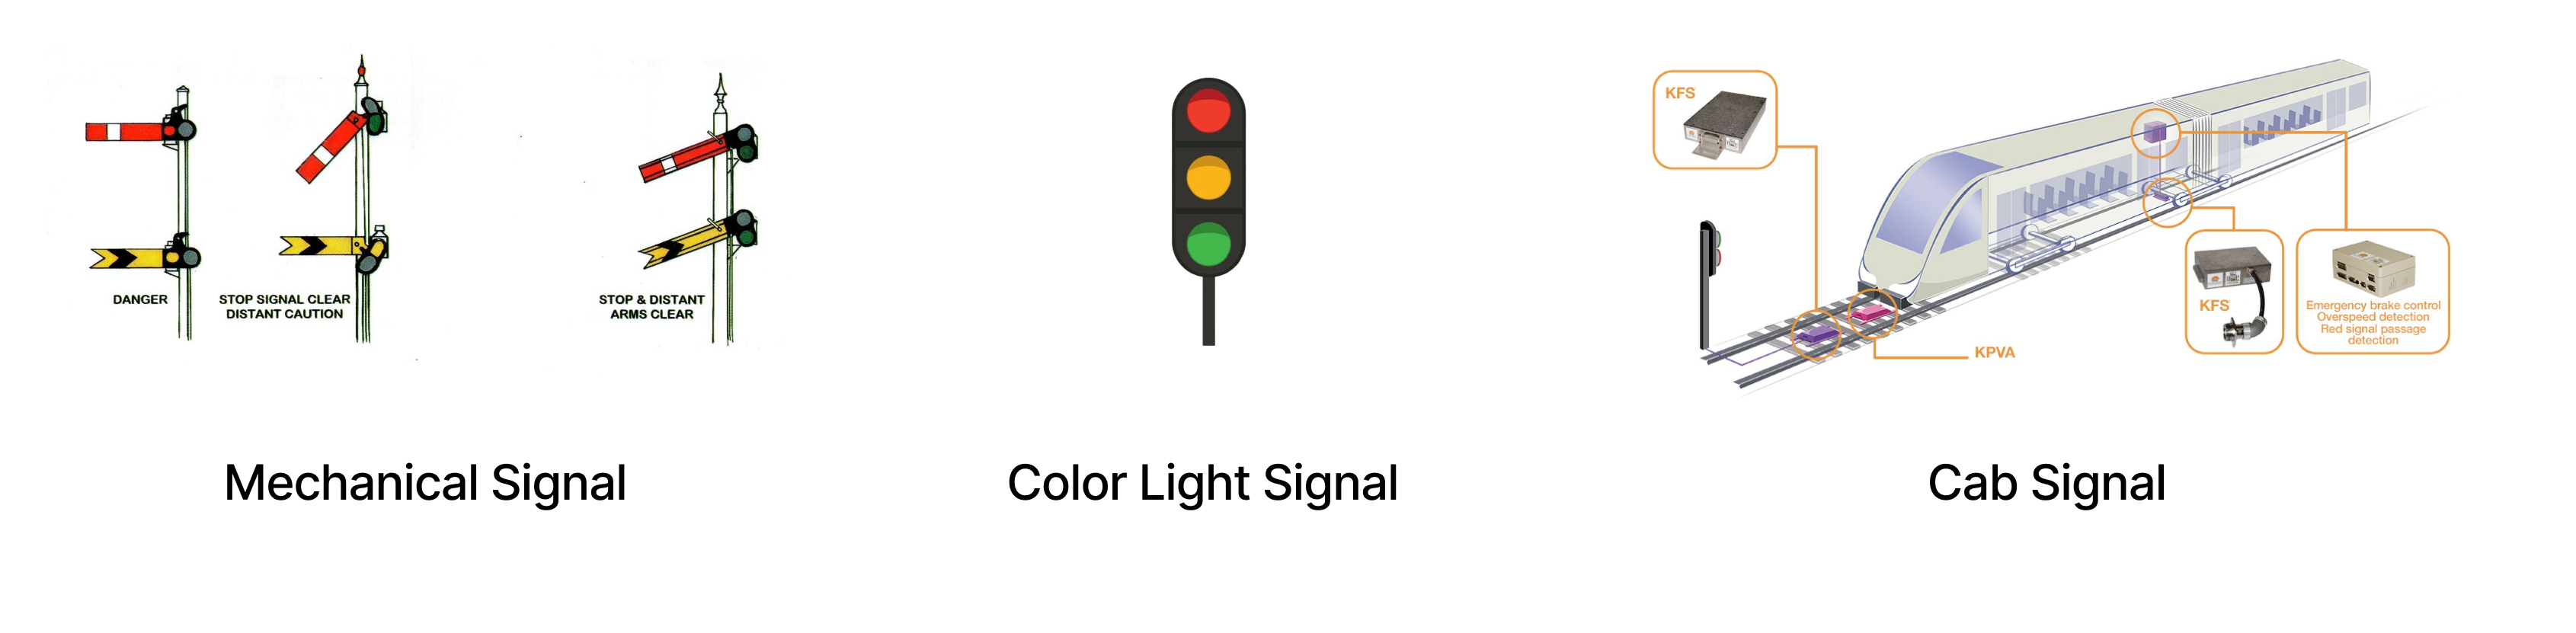
\includegraphics[width=1\textwidth]{images/signal-types/signalling_types.png}

    \floatcap{Different Signals}{Signals from left to right: Mechanical Signals, Color Light Signals, Cab Signal}
    
    \label{fig:signalling-types}
\end{figure}

While these mechanisms ensure safety, they often lack adaptability to real-time operational dynamics, especially in complex junctions or high-density corridors.
\section{Traditional Interlocking Methods}

Traditional interlocking systems have historically ensured railway safety by preventing conflicting train movements through physical or hardwired logic. While effective in their time, their rigidity and dependence on manual or fixed infrastructure limit their suitability for modern, high-density networks.

\subsection{Mechanical Interlocking}

Mechanical interlocking was the earliest form, relying on lever frames connected by rods and wires to points and signals. Safety was guaranteed through physical locking between levers, preventing operators from setting incompatible routes. This design provided robust fail-safe protection but came with drawbacks: it was labor-intensive, required large installations of levers and linkages, and depended on manual operation, making it slow and impractical for expanding or complex networks.

\subsection{Relay-Based Interlocking}

Relay-based interlocking replaced mechanical rods with electrical circuits, encoding safety conditions through electromechanical relays. This allowed greater automation, reduced manual workload, and increased reliability compared to mechanical systems. However, the logic was hardwired, meaning any change to track layout or operating rules demanded costly rewiring. Large relay rooms for busy stations also consumed space and required constant maintenance, limiting scalability as railway operations grew more dynamic.
\section{Computer-Based Interlocking (CBI)}

Computer-Based Interlocking (CBI) represents a fundamental shift from hardware-defined safety logic, such as relays or mechanical linkages, toward software-defined, programmable control. In a CBI, interlocking rules are expressed in software, often using high-level programming languages or specialized safety-certified platforms. This approach offers several advantages compared to traditional systems. Configurability becomes a key strength: rules can be updated, extended, or debugged without requiring physical rewiring or hardware replacement, significantly reducing cost and downtime. Scalability is also improved, as the same software framework can be adapted to different station layouts, operational policies, or national signaling practices. Another major benefit is the possibility of simulation-driven development—scenarios can be modeled and tested in a digital environment before deployment, allowing potential errors to be identified early. Finally, CBIs are inherently integration-ready, capable of interfacing with SCADA systems, traffic control centers, and modern IoT-based monitoring infrastructure, thereby enabling railways to operate as part of a larger, digitized transport ecosystem.

However, these advantages are balanced by significant challenges. The most critical is safety assurance, since shifting safety logic into software introduces risks of programming errors, unexpected interactions, or runtime faults. Unlike hardware logic, which is deterministic by design, software must be validated through rigorous verification pipelines, including formal proofs, redundancy strategies, and extensive field testing. Hardware dependency also poses risks, as failures in execution environments—such as operating system crashes, memory corruption, or processor faults—can compromise safety if not properly mitigated. Furthermore, CBIs must comply with demanding international standards, including EN 50128 for railway software and IEC 61508 for functional safety, which mandate strict processes for development, testing, and certification. Achieving compliance requires specialized expertise, documentation, and continuous auditing, often increasing both project cost and development time.

Despite these challenges, the global trend toward CBIs is accelerating, especially in regions seeking to modernize aging infrastructure without complete hardware overhaul. By combining flexibility, scalability, and digital integration with safety-critical assurance frameworks, CBIs are becoming the cornerstone of next-generation railway signaling.
\section{Review of Related Systems}
This section explores prominent interlocking systems that have shaped the industry and influenced our design.

\subsection{European Train Control System (ETCS)}
ETCS is a standardized signaling system under the European Rail Traffic Management System (ERTMS). It integrates interlocking with cab signaling and automatic train protection. ETCS Level 2 and 3 eliminate reliance on trackside signals, relying on continuous communication with onboard equipment. While highly advanced, it is cost-intensive and primarily suited for high-speed corridors.

\subsection{Solid State Interlocking (SSI)}
SSI was one of the first commercial microprocessor-based interlocking systems. Deployed in the UK and Europe, it uses a centralized computer to process logic and interface with relay interfaces. It demonstrated early benefits of programmability and space efficiency but was limited in graphical diagnostics and simulation support.

\subsection{Bangladesh Railway Practices}
Bangladesh Railways still predominantly relies on token-based or relay-based signaling, especially in non-electrified regions. While some modernization efforts have introduced computerized panels, the interlocking logic remains largely static and manually supervised. This environment highlights the need for cost-effective, software-centric solutions that are deployable in constrained settings.

\section{Standards and Reference Models}
To guarantee fail-safe operation, railway interlocking systems must conform to internationally recognized safety and engineering standards. These standards not only define technical requirements but also establish the processes, methodologies, and verification practices that ensure signaling systems achieve the highest levels of reliability and integrity.

\subsection{IEC 61508}
IEC 61508 serves as a foundational framework for the functional safety of electrical, electronic, and programmable systems across industries. Its significance lies in introducing the concept of Safety Integrity Levels (SILs), which quantify the probability of system failure and create a structured benchmark for reliability. Beyond classification, the standard emphasizes the importance of lifecycle management, ensuring that safety is considered at every stage of a system’s design, implementation, operation, and eventual decommissioning. For interlocking systems, IEC 61508 acts as the overarching reference, mandating redundancy strategies, fault-tolerant architectures, and rigorous testing protocols that underpin public confidence in railway operations.

\subsection{CENELEC EN 50126/50128/50129}
While IEC 61508 provides a general framework, the CENELEC standards—EN 50126, EN 50128, and EN 50129—translate these principles specifically into the railway domain. EN 50126 outlines the RAMS (Reliability, Availability, Maintainability, and Safety) lifecycle, requiring designers to address not only safety but also the long-term operational resilience of signaling systems. EN 50128 focuses on the software dimension, establishing stringent rules for coding practices, verification, validation, and configuration management. This is particularly relevant for modern computer-based interlocking, where software complexity directly influences safety outcomes. Finally, EN 50129 governs the approval process, bringing together hardware and software assurance to certify the complete system before it enters service. Together, these three standards ensure that railway interlockings are not only technically correct but also systematically verified, traceable, and certifiable in a regulatory environment.

\subsection{UML/SysML Modeling}
In addition to safety standards, contemporary practice increasingly leverages model-based systems engineering (MBSE) as a complementary reference framework. Unified Modeling Language (UML) and Systems Modeling Language (SysML) provide formalized ways to represent interlocking behavior, capturing route logic, state transitions, and failure responses in a structured and visual form. These models allow engineers to validate safety concepts in the early design stages, long before physical implementation, thereby reducing errors and accelerating certification processes. Beyond prototyping, UML and SysML also support traceability by linking safety requirements directly to system functions and test cases, ensuring alignment with the rigorous expectations of standards such as EN 50128. In this sense, modeling serves as a bridge between abstract safety requirements and concrete system design, reinforcing both technical clarity and compliance assurance.

\section{Gap Analysis}
Despite advancements in signaling, several shortcomings remain in traditional interlocking systems. High costs make modern vendor solutions inaccessible for many developing countries, leaving them dependent on outdated technologies. Relay and PLC-based systems also lack flexibility; adapting them to new layouts or operational changes often requires extensive rewiring, which limits scalability.

Another persistent issue is the absence of effective simulation tools. Without digital sandboxes, safety logic is difficult to test and validate before deployment, increasing risks during commissioning and restricting opportunities for operator training. Legacy systems are further constrained by poor integration with modern data-driven platforms, preventing their use in predictive maintenance or centralized control strategies.

Perhaps most critically, interlocking logic in conventional systems is opaque, often hidden within wiring or PLC blocks, making it difficult to audit, extend, or regulate. These limitations highlight the need for a modular, transparent, and software-defined approach that combines traditional safety robustness with the agility required in modern railway operations.


 \chapter{System Overview}
\label{chap:system-review}

\section{Overview}
\label{sec:system-overview:overview}

This system introduces a software-based approach to railway interlocking tailored for station-level control. Unlike traditional relay-based systems, this solution leverages a modular, rule-driven architecture that supports real-time logic evaluation, flexible customization, and safe automation of train movements.

The system aims to bridge the gap between rigid legacy systems and the demand for scalable, maintainable, and testable interlocking in developing regions. It does so by replacing static hardware rules with programmable safety logic, simulated validation, and dynamic route control.

\section{System Architecture}
\label{sec:system-overview:architecture}

The proposed interlocking system is structured into three interconnected layers, each with distinct responsibilities but designed to operate cohesively as part of a unified framework (illustrated in Figure~\ref{fig:top-level-view}). At the top sits the frontend operator interface, developed using Qt’s graphical framework. This interface provides dispatchers with a real-time, interactive view of the station layout, enabling them to issue route commands, monitor signal aspects and track occupancy, and receive immediate feedback on system status. Beyond its monitoring role, the frontend is designed with usability in mind, ensuring that complex interlocking operations can be executed quickly and reliably under the pressure of live railway operations.

\begin{figure}[t]
    \centering

    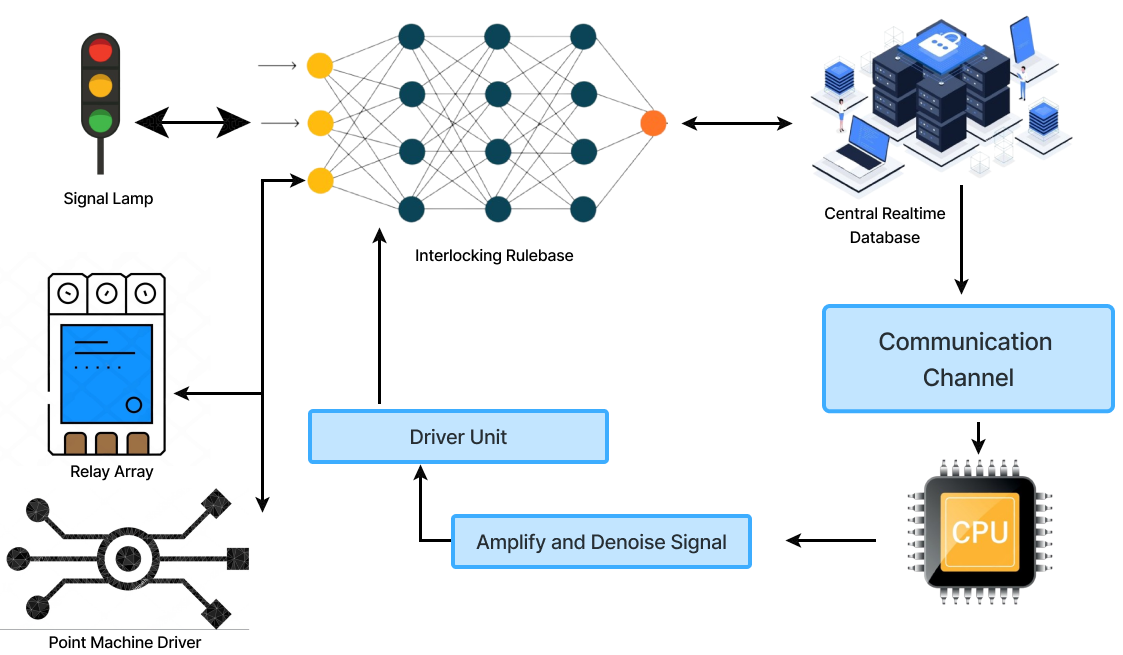
\includegraphics[width=0.85\textwidth]{images/architecture-diagrams/high-level-view.png}

    \floatcap{Top Level System Architecture}{This diagram illustrates how the major blocks of the system connected to each other.}
    
    \label{fig:top-level-view}
\end{figure}


Beneath the interface lies the backend logic engine, implemented in Qt C++. This core layer functions as the decision-making hub, executing interlocking rules, validating route requests, and coordinating the flow of events across the system. It encapsulates the safety logic, ensuring that all route settings and signal clearances conform to the constraints defined by interlocking principles. The engine is built with modularity in mind, allowing logic to be extended or reconfigured as operational needs evolve. Its reliance on Qt’s event-driven model, particularly signals and slots, enables asynchronous communication that preserves determinism while supporting real-time responsiveness.

At the foundation is the database layer, implemented on PostgreSQL. This layer manages both static configuration data, such as station topology and route definitions, and dynamic state data, including signal aspects, point machine positions, and track circuit occupancy. By consolidating both structural and operational information in a relational model, the database serves as the system’s single source of truth, enabling traceability, rollback functionality, and forensic analysis of past events. Its integration with database triggers and stored procedures also enhances fault tolerance by allowing critical validations to be enforced at the persistence level, creating a multi-layer safety net across the architecture.

Communication between these layers is facilitated through service interfaces, structured queries, and event emitters, following a loosely coupled service-based design. This architecture not only simplifies system extension and testing but also ensures resilience by isolating failures within individual layers. The result is a scalable and transparent interlocking framework that balances real-time performance with maintainability, making it adaptable for both simulation environments and future hardware-in-the-loop deployments.
\section{Core Components}
\label{sec:system-overview:components}

The interlocking system is composed of a set of modular components, each operating independently yet coordinated within the broader framework to ensure safe and reliable railway operations. At the operational level, the signal manager maintains continuous communication with the signaling elements, enforcing aspect control while defaulting all signals to “danger” unless safe conditions are validated. This not only aligns with fundamental safety principles but also ensures that the system is inherently fail-safe, minimizing risks during unexpected failures.

Equally critical is the point machine controller, which governs the alignment of switches and points before any route is authorized. By verifying that track elements are in the correct position, it guarantees route consistency and prevents conflicting train paths. The track circuit monitor complements this function by providing real-time feedback on track occupancy. Through constant surveillance of train positions, it identifies unauthorized entries into protected zones, creating a secondary safeguard against operational hazards.

At the center of the architecture lies the interlocking rule engine, which acts as the decision-making brain of the system. It evaluates route requests against predefined logical conditions, applying structured rules such as AND/OR combinations, overlap checks, and conflict resolution strategies. By blocking unsafe commands at the logic layer, it ensures that no single operator action or hardware anomaly can compromise system integrity.

These components are deliberately designed as reusable and testable modules, each capable of being validated in isolation. This modularity simplifies maintenance, supports incremental extension of functionality, and allows new configurations to be introduced without disrupting the stability of the overall system. Together, the components create a tightly integrated yet flexible framework that embodies both traditional safety assurances and the agility required for future expansions.
\section{Interlocking Logic Design}
\label{sec:system-overview:interlocking-logic}

At the heart of this system lies the rule engine — a modular processor of interlocking constraints encoded in a JSON-based configuration. Its responsibilities span a variety of logical checks required to authorize safe train movements and maintain route exclusivity.

The key logic handled by the engine includes route validation, point locking, overlap reservation, and support for conditional logic. These processes are dynamically loaded from station-specific configuration files, allowing flexible deployment without recompilation. Figure~\ref{fig:interlocking-logic-overview} illustrates a conceptual overview of surface level interaction among different interlocking modules. This includes inputs from track circuits, point machines, and signal requests, and how they funnel into a layered validation process.

\begin{figure}[t]
    \centering

    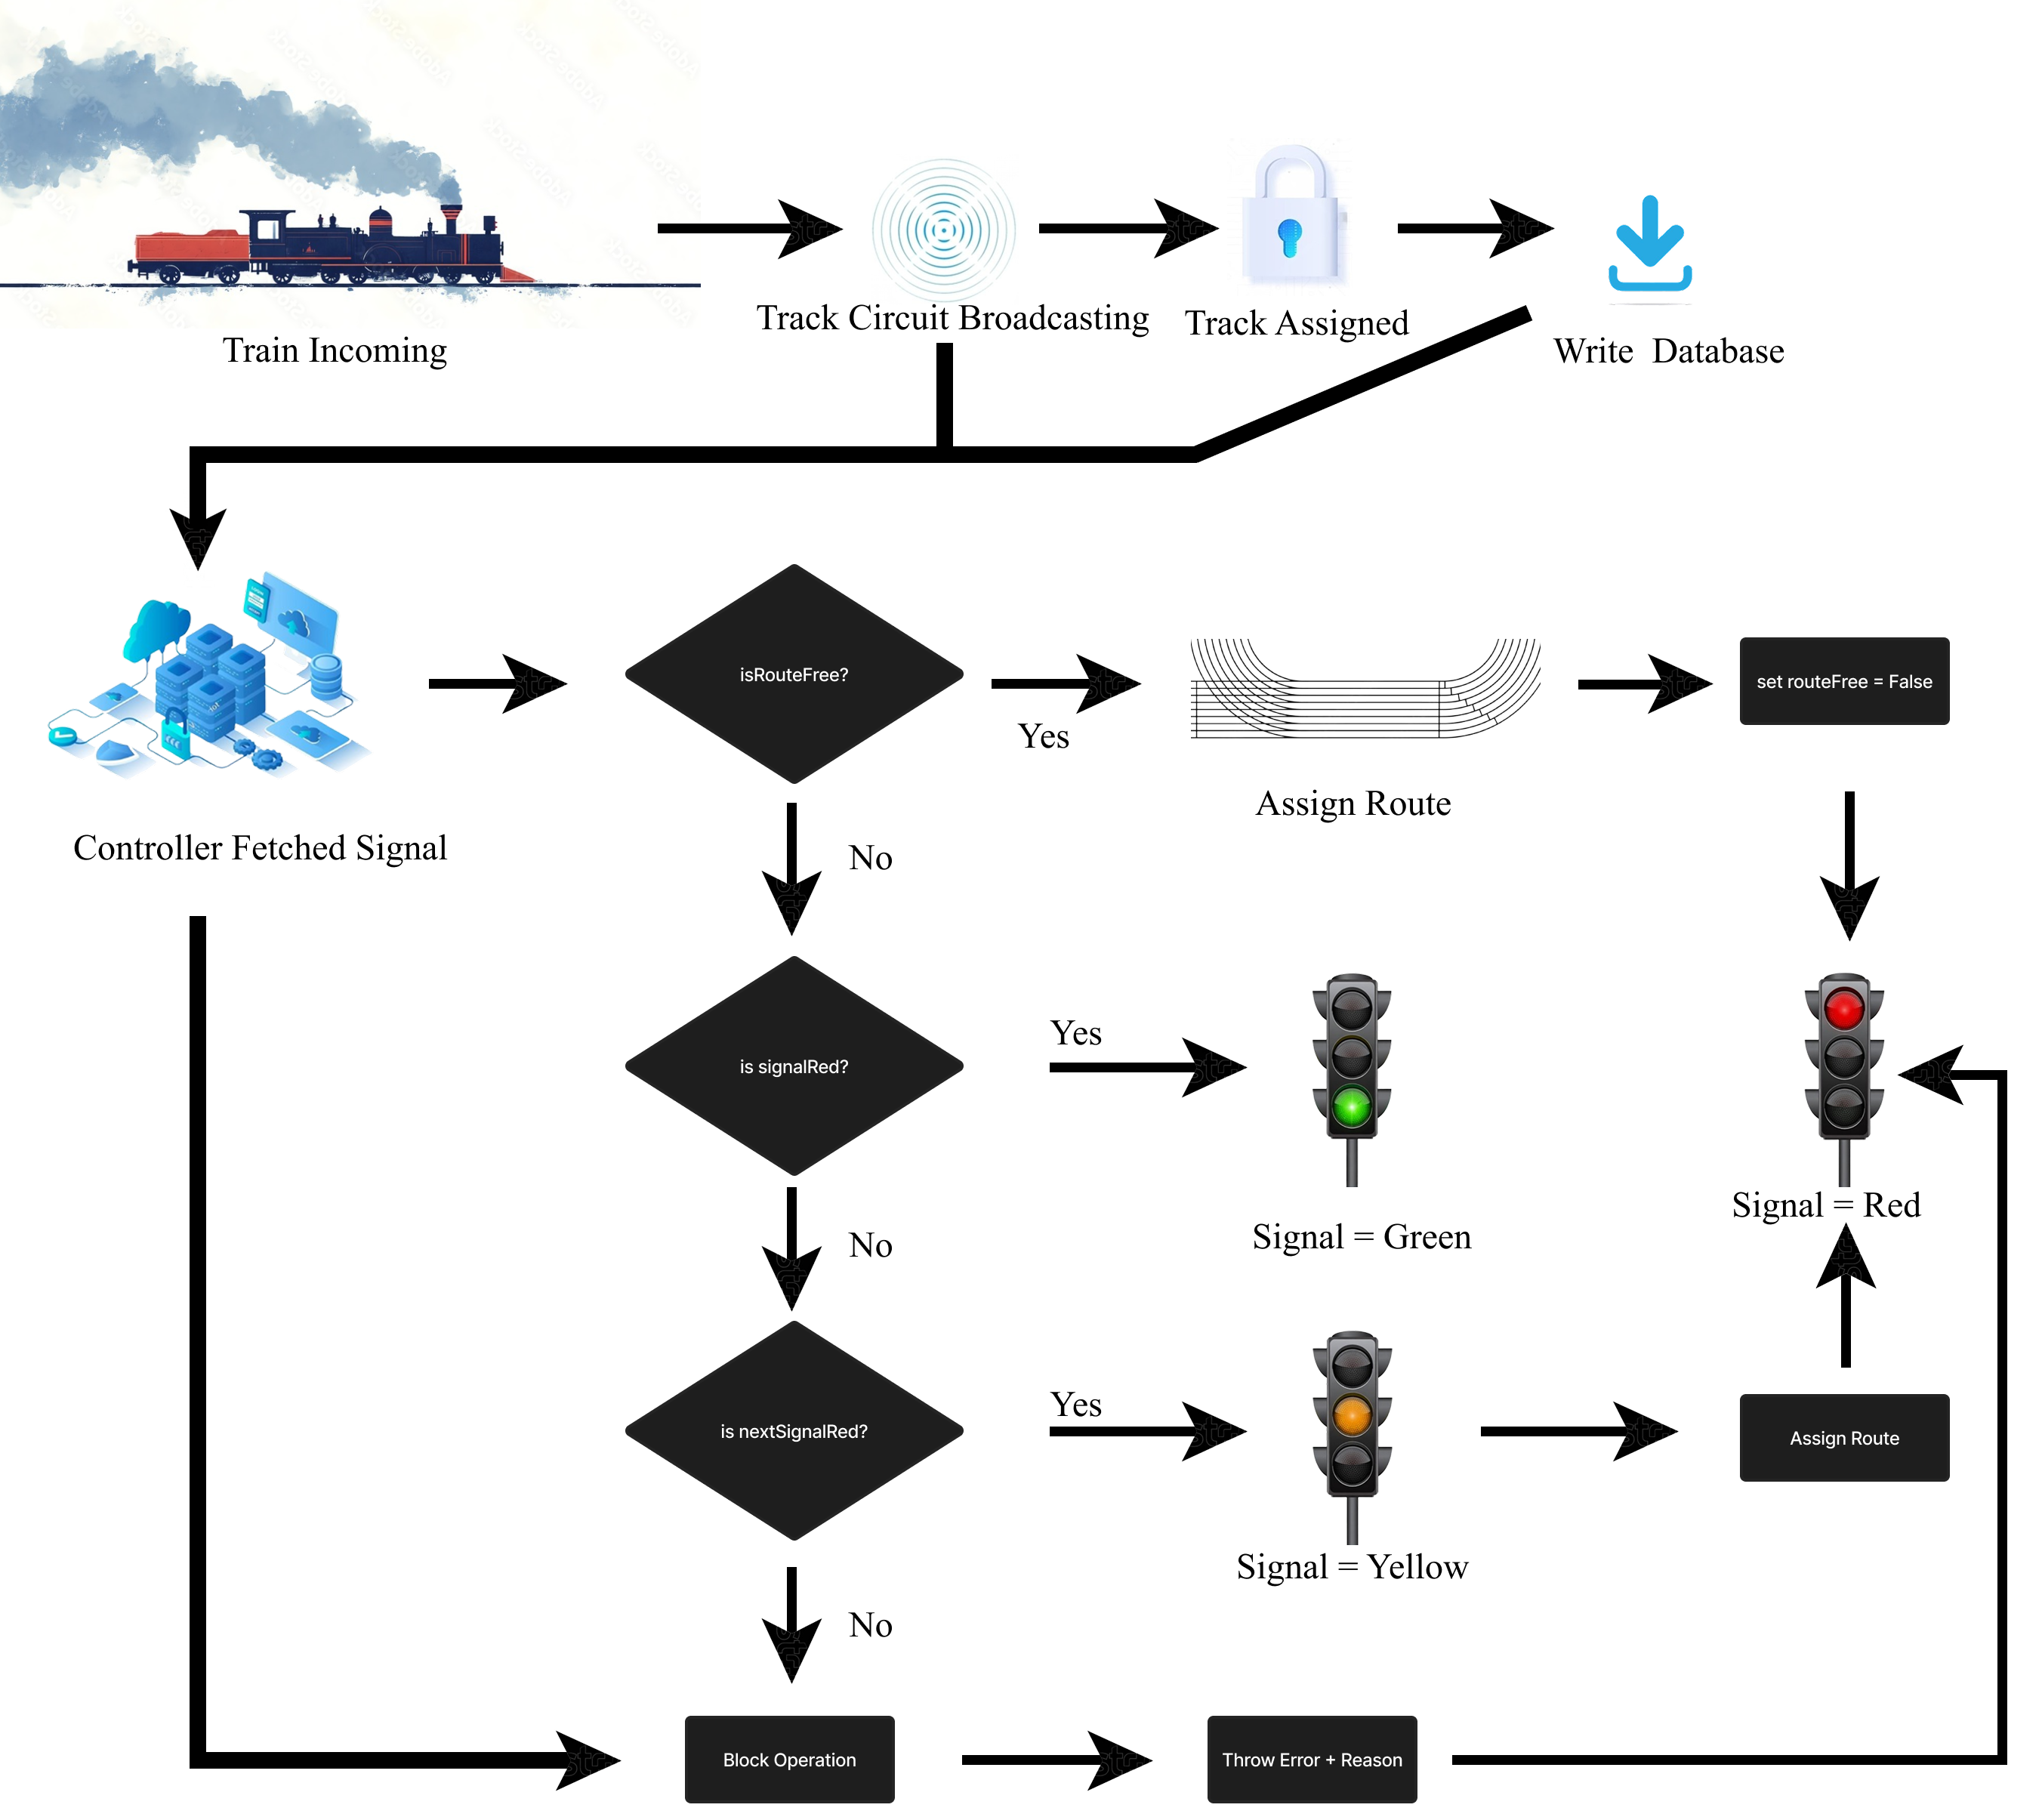
\includegraphics[width=0.85\textwidth]{images/interlocking-logic/interlocking_flow.png}

    \floatcap{Modular Interlocking Logic Flow}{Overview of validation layers including route conflict checks, point alignment, overlap safety, and conditional rule evaluation. These logic branches collectively ensure safe signal clearance.}
    
    \label{fig:interlocking-logic-overview}
\end{figure}


One of the most critical steps in this flow is route validation, where the system checks track segment occupancy, point alignment, and conflict-free paths. This process is discussed in detail in Section~\ref{sec:interlocking:route-validation} as a reference.

\section{Safety Mechanisms}

\label{sec:system-overview:safety}

Safety within the interlocking system is achieved through a layered approach that combines strict default behaviors with comprehensive validation checks. All signals are designed to default to “stop” unless explicitly proven safe, ensuring that no unintended clearance is ever granted. Before any command is executed, it must pass through multiple validation stages, including point alignment, route conflict detection, overlap availability, and flank protection. This multi-layer filtering ensures that errors or omissions in one area are caught by another, creating redundancy across the system.

In the event of a failure, detailed error logging and rollback mechanisms allow the system to revert to the last known safe state, preserving both operational continuity and forensic traceability. Even manual interventions are subject to the same safety logic, preventing unsafe overrides and maintaining consistency between automated and human actions. By structuring these mechanisms to withstand single points of failure, the system upholds the core principle of interlocking: that safety must never be compromised, regardless of the circumstances.
\section{Operational Workflow}
\label{sec:system-overview:workflow}

Figure~\ref{fig:interlocking-logic-overview} outlines the interaction between components during a typical signal command.

When an operator initiates a command through the user interface, the system first retrieves real-time information on track occupancy, point machine positions, and current signal aspects. This data is then passed to the interlocking rule engine, which evaluates route availability, overlap zones, and all relevant safety constraints. Only if every condition is satisfied is the signal cleared and the associated points locked in place to protect the movement authority. In cases where validation fails, the system responds immediately with a diagnostic message, explaining which requirement was not met. This structured process not only enables confident and transparent decision-making but also provides complete traceability, ensuring that every action can be audited and analyzed in the event of an irregularity or system failure.


 \chapter{Interlocking Logic Design}
\label{chap:interlocking-logic}

\section{Route Validation Rules}
\label{sec:interlocking:route-validation}

Route validation is the first and most critical step before granting authority for any train movement. It ensures that a requested path complies with all operational and safety constraints defined within the interlocking schema. To achieve this, the system evaluates the availability of every track segment along the route, confirming that no section is already occupied. It simultaneously checks for potential conflicts with active or pending paths to guarantee that no intersecting movements are permitted. The validation also extends to point machines, verifying that each one is correctly aligned and locked in its designated position. At the route’s endpoint, an additional safety requirement is enforced by reserving an overlap zone, effectively providing a braking buffer should the train fail to stop as expected.

All validation rules are maintained in station-specific JSON files that are parsed dynamically by the rule engine. This separation of rules from the codebase enhances flexibility, allowing adjustments or extensions without invasive software changes. In cases where any validation check fails, the route is immediately rejected, and the outcome is logged for full traceability. These logged results not only aid in diagnostic review but also form the foundation for subsequent signal aspect decisions, as detailed in Section~\ref{sec:interlocking:signal-decision}.
\section{Signal Aspect Decision Logic}
\label{sec:interlocking:signal-decision}

Once a route has been successfully validated and reserved, the system determines the appropriate signal aspect to display. This decision logic enforces the safe representation of signal colors, ensuring that the displayed aspect always reflects both the status of the authorized route and the occupancy of downstream track sections. A signal will only clear if the associated route passes all safety checks and the next block is confirmed as free; otherwise, it remains at danger. Conditional interlocking is also considered, where dependencies on adjacent signals, track circuits, or point machines may influence the final decision.

The resulting output is expressed through the standard aspects of red, yellow, or green. Red represents the default and inherently safe condition, indicating that movement is not permitted. Yellow serves as a cautionary aspect, warning the driver that the train may proceed but must be prepared to stop at the next signal, often because the following block is occupied. Green conveys full clearance, authorizing the train to proceed at the permitted speed with assurance that the track ahead is safe. These updates are continuously processed by the Qt backend and rendered in real time on the graphical operator interface, providing both operators and drivers with immediate, unambiguous feedback on network status.

\section{Conditional Control Modes}
\label{sec:interlocking:control-modes}

To handle complex station layouts and shared infrastructure, the interlocking engine incorporates flexible control modes that allow rules to be enforced with varying levels of strictness. In some cases, absolute conditions must be satisfied—such as when multiple track elements or safety requirements need to align precisely—ensuring the highest level of security for critical routes. In other scenarios, the system permits fallback logic, where meeting one of several defined conditions is sufficient. This is particularly valuable when alternate overlaps or redundant paths are available, allowing safe continuity of operations even if the primary option is unavailable.

These modes are configured on a per-rule basis within the JSON schema, giving engineers the ability to fine-tune interlocking behavior without altering the core code. By supporting both strict and permissive logic patterns, the system balances safety with operational flexibility, ensuring that rules remain both robust and adaptable to the realities of diverse railway environments.
\section{Overlap Protection Handling}
\label{sec:interlocking:overlap-protection}

Overlaps are reserved track segments positioned beyond a signal, serving as a critical safety buffer should a train overshoot its intended stopping point. The system enforces overlap protection through both static and dynamic modes. In static configurations, each route is assigned a predefined overlap that must be proven unoccupied and securely locked before the signal can clear. In dynamic mode, the interlocking engine selects from a list of candidate overlaps and reserves the first available option, ensuring flexibility in complex station layouts. Once granted, an overlap remains locked until the train has fully cleared it, as confirmed by occupancy sensors, after which it is released back into operation. If no valid overlap can be secured, the requested route is denied and the signal remains at red. By enforcing this mechanism, the system provides a crucial safeguard against accidents arising from emergency braking failures or wheel slippage, ensuring that even unexpected overruns remain contained within a controlled and protected zone.

\section{Safety Checks and Conflict Detection}
\label{sec:interlocking:safety-checks}

Safety is not enforced by a single rule but by a layered mechanism of pre-validation, real-time monitoring, and fallback measures. The interlocking system includes:

\begin{itemize}
\item \textbf{Route Conflict Detection:} Base engine can detect and pinpoint conflicting sections. Ensures no two active routes share track segments. A lookup against all reserved routes is performed before a new route is committed.
\item \textbf{Point Conflict Detection:} Prevents contradictory point commands. A point cannot be locked in two opposing positions simultaneously across overlapping routes.
\item \textbf{Occupancy Synchronization:} Real-time updates from track circuits ensure stale or conflicting data does not lead to unsafe decisions.
\item \textbf{Command Verification:} Each command (e.g., route reservation, point alignment) passes a verification layer before execution.
\item \textbf{System Logs and Feedback:} Any blocked or failed operation is logged with reasons and presented to the operator via the UI.
\end{itemize}

The safety framework has been designed to align with best practices in software-defined safety systems (IEC 61508, EN 50128), though full certification is marked as future work.


\chapter{Methodology}
\label{chap:methodology}

\section{Interlocking Service Module}
\label{sec:methodology:interlocking-service}

The InterlockingService module acts as the central coordinator between operator or system-initiated requests and the underlying safety branches. It governs the lifecycle of interlocking operations, beginning with the initialization of validation logic, through rule execution, and into reactive safety enforcement. By supervising dedicated branches for signals, point machines, and track circuits, the service consolidates their outputs into a single validation result, ensuring consistency across the system. This result not only determines whether a route or signal request may proceed but also provides reason-tagged feedback for both the operator interface and the system logger, reinforcing transparency and accountability.

Inputs to the service may originate from a variety of sources, including the operator GUI, automated testing scripts, or the simulation environment. Once received, these requests are interpreted against current infrastructure states retrieved from the database, after which the service coordinates validation checks across the relevant modules. The outcome is then disseminated in real time: updates are reflected on the graphical simulation panel, logs are recorded for traceability, and, where necessary, alerts or freeze events are triggered to contain unsafe conditions.

The design emphasizes modularity, responsiveness, and resilience. Validation logic is branch-based, ensuring that point, track, and signal rules remain cleanly separated and individually testable. Performance is benchmarked so that even under heavy operational loads, the service can respond within real-time constraints. Reactive safety is also embedded: changes in track occupancy immediately trigger enforcement logic, enabling the system to respond dynamically to unexpected events. In this role, the InterlockingService functions as the orchestration layer of the interlocking system, binding together the rule engine, validation modules, and operator interface into a coherent and fail-safe whole.
\section{Interlocking Rule Engine Module}
\label{sec:methodology:rule-engine}

The InterlockingRuleEngine is the central validation engine responsible for enforcing the rules that govern signal aspect transitions. It operates by loading declarative logic from structured JSON files, parsing control relationships and conditions independently of the codebase, and then evaluating requests against live infrastructure data obtained through the DatabaseManager. This separation of configuration from implementation provides significant flexibility, allowing safety rules to be updated or extended without recompilation and ensuring that domain experts can refine logic directly at the schema level.

When a signal aspect change is requested, the engine applies a multi-stage evaluation process. It determines whether the signal is independent or subject to control by other signals, validates the status of track circuits and point machines, and checks that all defined conditions are satisfied. The system then aggregates these results according to the defined control mode, applying either strict or permissive logic as specified. The outcome is returned as a validation result object that records the decision, the reasoning behind it, and any affected infrastructure, ensuring that operators and auditors retain full visibility into the decision-making process.

The design of the engine emphasizes modularity, with dedicated components for parsing, evaluation, and database access. Diagnostic logging is embedded throughout, allowing each validation step to be reconstructed for debugging or forensic analysis. By combining declarative rule definition with modular execution, the InterlockingRuleEngine ensures that interlocking logic remains transparent, adaptable, and verifiable—qualities that distinguish it from the rigid, hardwired behavior of relay or PLC-based systems.
\section{SignalBranch Module}
\label{sec:methodology:signal-branch}

The SignalBranch module is dedicated to validating and enforcing signal-specific logic whenever a route request is initiated. Its core responsibility is to ensure that the conditions tied to each signal aspect are satisfied before a signal is cleared for train movement. This involves evaluating whether a signal can safely display a permissive aspect, such as green or yellow, based on the current rules and real-time infrastructure states. To achieve this, the module interacts with track circuit data, point machine positions, and defined rule dependencies, ensuring that signals only transition when the entire route has been validated as safe.

The logic flow is tightly integrated into the broader InterlockingRuleEngine, which invokes the module’s validation methods as part of the signal clearance process. Inputs are drawn from live track occupancy updates provided by the TrackCircuitBranch and consolidated into structured validation results that feed both the system logger and the operator interface. This design ensures that every clearance decision is traceable, both visually in the simulation layer and persistently through event logs.

The module was deliberately designed with modularity and extensibility in mind. By treating signals as independent units with their own configurable rules, changes in signaling logic can be made without disrupting the broader system. Abstraction layers separate signal validation from track and point logic, while JSON-based configurations allow dependencies to be expressed through flexible AND/OR conditions. This approach minimizes code changes while preserving adaptability, making the SignalBranch both a reliable enforcer of safety and a flexible component for evolving station requirements.
% Optional:
% \begin{figure}[H]
%     \centering
%     \includegraphics[width=0.85\textwidth]{images/module-flow/signal-branch-flow.pdf}
%     \floatcap{Signal Branch Flowchart}{Illustration of signal validation process through SignalBranch}
%     \label{fig:signal-branch-flow}
% \end{figure}

\section{Point Machine Branch}
\label{sec:methodology:point-machine-branch}

The PointMachineBranch module is responsible for validating point machine operations and ensuring that any requested movement between NORMAL and REVERSE positions is carried out safely. Point machines serve as critical mechanical switches that guide trains across diverging tracks, and their reliability is essential to prevent derailments or route conflicts. Before a position change is permitted, the module evaluates a range of safety checks, confirming that the machine exists and is active, that the requested position differs from the current one, and that the device is not mechanically or time-locked. It further verifies that all guarding track segments are unoccupied, associated protective signals display red, and no conflicts exist with neighboring points or active routes. Only if all conditions are satisfied will the operation be approved.

The module receives input such as the point machine identifier, its requested state, and real-time operational data retrieved through the DatabaseManager. It also references metadata linking the point to track topology and checks signal states to enforce protective locking. Integrated directly into the InterlockingRuleEngine, the PointMachineBranch is invoked whenever a route request involves a point movement, whether in live operation or simulation scenarios.

Diagnostics are embedded throughout the validation process. Each stage is logged with precise timestamps, reasons for approval or rejection, and references to affected entities. These logs support both real-time troubleshooting and forensic analysis of interlocking behavior, making it easier to trace the root causes of violations or timing conflicts. For instance, if point machine PM07 is requested to move from NORMAL to REVERSE, the module ensures it is active, not already in REVERSE, not locked, and that the connected track segments are clear before returning an ALLOWED result. If any condition fails, a BLOCKED response is generated along with a detailed explanation, reinforcing both operational safety and system transparency.
\section{Track Circuit Branch}
\label{sec:methodology:track-circuit-branch}

The TrackCircuitBranch module enforces automatic safety responses whenever a track segment’s occupancy status changes. When a segment transitions from clear to occupied, the module immediately identifies all associated protecting signals and commands them to display the RED aspect, ensuring that no conflicting train movement can occur. This direct coupling between track detection and signal enforcement embodies one of the most fundamental principles of interlocking: occupied tracks must always be safeguarded by restrictive signals.

The validation process begins by confirming the existence and active status of the occupied segment before retrieving its protecting signals from database metadata and configuration tables. Once identified, these signals are forcefully set to danger and logged for traceability. If the system detects an anomaly—for example, a failure to update one of the signals—the module escalates the response by emitting freeze signals and generating diagnostic entries with timestamps and reasons for failure. This layered enforcement not only guarantees immediate protection but also preserves the forensic trail needed for post-event analysis.

Integration with the broader interlocking engine is seamless. The module is automatically triggered by occupancy monitoring services and backend processes that supervise train movements across the network. Its outputs are reflected simultaneously in the simulation environment, operator interface, and persistent audit layers, ensuring that both real-time operations and long-term compliance requirements are satisfied. For instance, when track segment T22 becomes newly occupied, protecting signals such as S13 and S14 are instantly forced to red. If one fails to respond, the system transitions into a safe freeze state, with detailed logs capturing every step of the enforcement.

Through this design, the TrackCircuitBranch acts as the reactive guardian of the interlocking system, ensuring that the fundamental link between track detection and signal protection is never broken, even in the presence of faults or unexpected conditions.
\section{SignalRule Module}
\label{sec:methodology:signal-rule}

The SignalRule module encapsulates the interlocking logic associated with a specific signal aspect condition, defining the circumstances under which a controlling signal permits another signal to display a given aspect. Each rule holds the necessary dependencies—such as track occupancy, point machine alignment, or protecting signal states—and provides methods to evaluate whether a requested aspect transition is allowed. By isolating these conditions into discrete rule objects, the system maintains modularity, enabling individual rules to be updated or extended without altering the overall engine.

When a validation query is initiated, the rule evaluates its stored conditions and determines whether the target signal may safely assume the requested aspect. To improve runtime efficiency, the module employs an internal cache that maps signal identifiers to their permitted aspects, reducing the overhead of repeated lookups during high-frequency operations. This approach ensures that real-time performance targets are maintained even in complex station environments with numerous signals and overlapping dependencies.

Integration with the InterlockingRuleEngine is seamless: rules are constructed from parsed JSON data and executed dynamically during validation cycles. Their outcomes feed into the broader validation framework, producing structured results that include both the decision (allowed or blocked) and the reasoning behind it. This explicit traceability supports debugging, audits, and compliance with safety standards, while the separation of rule logic from the core engine reinforces modularity and long-term maintainability. In practice, the SignalRule module serves as the building block of declarative interlocking logic, bridging abstract configuration data with executable safety enforcement in a clear and efficient manner.

 \chapter{Implementation}
\label{chap:implementation}

\section{Technology Stack}
\label{sec:implementation:tech-stack}

The system is implemented on a modern, cross-platform technology stack optimized for real-time control, maintainability, and extensibility. At its core, Qt with C++ provides both the backend logic and the graphical interface, leveraging its signal-slot architecture to ensure asynchronous communication and deterministic event handling. This is complemented by QML, which extends the framework with a flexible and animated simulation environment, allowing operators and developers to visualize interlocking behavior dynamically. Persistent data management is handled through PostgreSQL, which maintains normalized representations of both static infrastructure and runtime interlocking states, ensuring consistency and traceability. Build processes are coordinated through CMake, enabling reproducible configurations and streamlined compilation across platforms. Together, these technologies form a cohesive ecosystem that tightly integrates logic processing, data persistence, and visualization—an essential combination for an interlocking system where safety, usability, and adaptability must coexist seamlessly.

\section{Database Schema (PostgreSQL)}
\label{sec:implementation:database-schema}

The PostgreSQL schema is structured to represent railway infrastructure in a way that supports real-time interlocking validation, efficient querying, and strict audit compliance. It is organized into three logical namespaces: one dedicated to core control entities such as signals, track segments, and point machines; another for configuration data like signal types, aspects, and point positions; and a third reserved for audit logging of operational events, state transitions, and safety checks. This separation not only improves maintainability but also ensures that logic, configuration, and oversight remain clearly distinct.

The schema is further optimized for flexibility and performance through the use of JSONB fields, GIN indexes, and array structures, allowing complex rules and state data to be represented in a compact and query-efficient manner. Real-time responsiveness is achieved with database triggers and the pg\_notify mechanism, which broadcast updates to critical control elements as they occur. At the same time, embedded audit logging ensures that every operational decision and safety-relevant change is captured with full traceability, meeting the demands of regulatory oversight. By combining circuit-based occupancy tracking with these advanced features, the schema provides both the precision needed for safe operations and the extensibility required for long-term evolution.
\section{Rule Engine Implementation (Qt C++)}
\label{sec:implementation:rule-engine}

The interlocking rule engine is implemented as a modular core component, deliberately decoupled from the graphical interface to ensure that safety-critical logic remains robust and independent of user-facing states. Its architecture is organized around specialized validation branches, each responsible for a distinct operational domain such as track clearance, point machine alignment, overlap availability, and signal dependencies. By delegating these checks to independent modules, the engine maintains both clarity of responsibility and ease of future extension.

When a request is made to clear a signal or reserve a route, the engine retrieves the relevant rule from the database and evaluates it against current infrastructure states. The process integrates multiple conditions in parallel, and the outcome is encapsulated in a structured validation result that either authorizes the command or records explicit reasons for rejection. This design not only enforces rigorous safety constraints but also provides transparency and traceability for operators and auditors. The layered approach reflects modern software engineering principles, allowing the rule engine to evolve without compromising its core function as the guardian of safe train movement.
\section{Logging and Debugging Tools}
\label{sec:implementation:logging-debugging}

Comprehensive logging is essential for safety validation, operational transparency, and post-event analysis in an interlocking system. The proposed framework adopts a multi-tiered approach that captures events with varying levels of detail, ensuring that both real-time monitoring and long-term auditing needs are met. At the backend level, every interlocking decision—such as a signal clearance or a rejected route request—is timestamped with its input parameters and validation outcomes, guaranteeing complete traceability of operational behavior. Structured logs are stored in dedicated database tables, where fields capture component identity, action taken, status, and any associated failure reason. This structured format allows efficient querying for audits, diagnostics, and compliance checks.

During development and simulation, the system leverages Qt’s console utilities to provide categorized diagnostic messages. Routine updates are emitted as standard debug logs, warnings highlight unexpected but non-critical anomalies, and critical errors are flagged immediately to indicate failed safety validations or major exceptions. This real-time feedback accelerates troubleshooting by giving engineers immediate insight into system behavior under different conditions.

Beyond live debugging, the logging infrastructure is equally important for post-mortem analysis. By reconstructing event sequences from historical logs, engineers can validate whether safety logic responded correctly under stress or identify where faults originated. This dual role—supporting both immediate debugging and long-term accountability—ensures that the interlocking system remains transparent, verifiable, and aligned with the rigorous demands of railway safety.
\section{Simulation Interface}
\label{sec:implementation:simulation-interface}

A visual simulation interface was developed to function both as a verification platform for engineers and a training tool for operators. Using QML and SVG technologies, it renders the station layout with dynamic overlays that animate train movements, point machine states, and signal aspects in real time. This allows interlocking decisions from the backend engine to be presented visually, making it possible to confirm system behavior under various operational scenarios. Signals transition through standard aspects, switches animate to reflect alignment and lock status, and train icons traverse routes as occupancy data updates, providing an intuitive representation of safety logic in action.

Beyond its engineering role, the interface serves as an accessible demonstration tool for stakeholders. Operators can select routes through the control panel, observe how validation is performed by the rule engine, and follow simulated train movements across track segments while logs are generated in parallel. This combination of visualization and data traceability makes the platform valuable not only for technical debugging but also for communicating safety principles to administrators and training personnel. By bridging the gap between backend logic and user understanding, the simulation interface enhances both confidence in the system and the effectiveness of operator training.

 \chapter{Case Study: Example Layout}
\label{chap:example-layout}

\section{Layout Description}
\label{sec:example-layout:description}


\section{Rule Definition Samples}
\label{sec:example-layout:rules}


\section{Signal Operation Scenarios}
\label{sec:example-layout:scenarios}


\section{Failure Cases and Safety Responses}
\label{sec:example-layout:failures}



 \chapter{Results}
\label{chap:Results}

\section{Evaluation Methodology}
\label{sec:evaluation:methodology}

\section{Test Cases and Scenarios}
\label{sec:evaluation:test-cases}


\section{System Performance}
\label{sec:evaluation:performance}

Performance evaluation focused on the system’s ability to handle real-time interlocking tasks under concurrent load. Key benchmarks are summarized below:

\begin{itemize}
    \item \textbf{Average Rule Evaluation Time:} 12 milliseconds
    \item \textbf{Signal Command Response Latency:} < 50 milliseconds
    \item \textbf{Concurrent Route Handling Capacity:} Up to 50 route requests/second
    \item \textbf{Startup Initialization Time:} < 300 milliseconds
\end{itemize}

These results affirm the system's suitability for deployment in small to medium-sized stations, where quick decisions and responsiveness are critical. Performance was consistent across repeated runs and different topological configurations.

\section{Safety and Reliability}
\label{sec:evaluation:reliability}


\section{Limitations}
\label{sec:evaluation:limitation}



 \chapter{Societal, Health, Environment, Safety, Ethical, Legal and Cultural Issues}
\label{chap:outro}

\section{Intellectual Property Considerations}
\label{sec:outro:property}

The development of a modular, software-based interlocking system raises significant intellectual property (IP) considerations, particularly because it redefines a traditionally hardware-bound safety domain into an adaptable, software-driven framework. Unlike conventional relay or PLC-based interlockings, which are often encumbered by vendor lock-in, the proposed design shifts innovation toward programmable, database-driven safety logic. This change requires careful attention to the ownership of algorithms, data structures, and rule-engine configurations.

In the context of Bangladesh, where railway modernization efforts often rely heavily on foreign vendors, ensuring local ownership of the intellectual assets is particularly important. The declarative rule engine, simulation framework, and integration workflows developed in this thesis can be seen as national assets, providing the foundation for domestic expertise in railway safety technologies. Protecting such assets—through patents, copyrights, or institutional agreements—helps to prevent unlicensed replication and ensures that the benefits of innovation accrue locally rather than being appropriated by external contractors.

Additionally, the open-ended nature of software interlocking systems creates a tension between standardization and proprietary control. While railway safety logic must conform to international safety standards (e.g., EN 50128), the implementation details—such as modular rule evaluation, hybrid database triggers, or simulation interfaces—carry distinct intellectual value. Proper licensing and IP protection mechanisms are therefore essential to strike a balance between open collaboration for safety and protection against exploitation by third parties.
\section{Ethical Considerations}
\label{sec:outro:ethics}

Ethical considerations in railway safety systems are not limited to technical correctness but extend to fairness, transparency, and accountability in design and deployment. An interlocking system directly governs life-critical operations; ethical responsibility therefore demands that the system be transparent in its decision-making, traceable in its error reporting, and resilient against misuse or negligence.

For Bangladesh, where railways are often under pressure from high passenger density and constrained infrastructure, ethical responsibility also includes addressing the societal equity of safe access to transport. A failure in interlocking logic disproportionately affects vulnerable communities who rely on affordable railway transport. Designing a system that minimizes downtime, reduces human error, and ensures consistent application of safety rules contributes directly to the ethical principle of safeguarding human life.

At the same time, ethical dilemmas may arise when balancing cost constraints with safety-critical investments. Software-based solutions must not be viewed merely as low-cost alternatives but as ethically grounded systems that uphold, or even surpass, the safety benchmarks of traditional relay or PLC-based interlockings. Ethical practice also includes ensuring proper training for operators, avoiding hidden biases in configuration (e.g., favoring certain routes or services), and maintaining transparency with regulators and stakeholders about the system’s capabilities and limitations.
\section{Safety Considerations}
\label{sec:outro:safety}

Safety is the central pillar of any interlocking system, and the proposed software-based design must meet or exceed the expectations of fail-safe operation defined in global railway safety standards. In practice, this requires multiple overlapping layers of defense: validation cascades, rollback mechanisms, formal error logging, and system freeze protocols that act as safeguards against unsafe states. Unlike legacy interlockings where safety is “hard-wired” into electromechanical logic, this system relies on the correctness and integrity of software modules, making rigorous testing and verification indispensable.

In the Bangladeshi railway context, additional challenges arise from infrastructural variability, maintenance gaps, and environmental stressors such as humidity and seasonal flooding. Safety considerations must therefore include robust error detection under imperfect conditions, graceful degradation in the event of hardware or network failures, and clear recovery paths when abnormal events occur. The simulation and HIL capabilities built into the system are not just technical enhancements but essential safety measures, enabling continuous operator training, pre-deployment testing, and forensic analysis of incidents.

Furthermore, safety is inseparable from organizational processes. The role-based access control model ensures that unauthorized interventions are prevented, reducing risks from both negligence and malicious actions. Real-time monitoring and logging also provide accountability, allowing regulators and engineers to trace the sequence of operations leading to any disruption. In this way, the system’s architecture embodies a safety philosophy that goes beyond compliance, aiming to embed reliability and trustworthiness into everyday railway operations.
\section{Legal Considerations}
\label{sec:outro:legal}

Legal considerations for a software-based interlocking system center on compliance with railway safety standards, liability, and data governance. Unlike traditional relay-based systems, a modular software approach must adhere to frameworks such as CENELEC EN 50128 and EN 50129, which carry both technical and legal weight in certifying safety-critical applications. For Bangladesh, adopting such standards ensures credibility and compatibility with international partners.

Liability is another critical issue, since any system malfunction could lead to severe accidents. Clear legal responsibility must be established among developers, operators, and regulators, particularly as local certification structures for software safety are still emerging. The system’s logging and forensic features also have legal implications, as records may be required in accident investigations; ensuring their authenticity and secure storage is therefore essential.

Finally, procurement and licensing laws shape how locally developed solutions are owned and deployed. Proper agreements are needed to prevent disputes over code ownership and to safeguard national control over future system development. Integrating these legal safeguards from the outset strengthens both the reliability and acceptance of the interlocking solution.
\section{Impact of the Project on Societal, Health, and Cultural Issues}
\label{sec:outro:social}

\subsection{Social Impact}
The modernization of railway interlocking through a locally developed, software-based system has a direct societal benefit by strengthening a mode of transport that serves millions of people daily in Bangladesh. Reliable signaling reduces delays, minimizes human error, and enhances passenger confidence in public transport. In a country where many communities depend on railways for affordable mobility, improved efficiency translates into better access to education, employment, and commerce. Furthermore, reducing dependency on foreign vendors supports technological self-reliance and fosters national capacity building, which has long-term societal implications for infrastructure independence and skill development within the local workforce.

\subsection{Health Impact}
Railway safety is inherently tied to public health outcomes. Signal failures or mismanagement can result in accidents that cause injuries and loss of life on a large scale. By embedding multi-layer safety validations, error logging, and real-time monitoring, the system contributes to accident prevention and emergency preparedness. Beyond direct passenger safety, improved railway reliability also impacts health indirectly—by encouraging the use of rail transport over road alternatives, it can reduce traffic congestion and vehicular pollution, both of which have long-term health effects on urban populations. A safer and more dependable railway network thus becomes an enabler of healthier, more sustainable living conditions.

\subsection{Cultural Impact}
Railways hold deep cultural significance in Bangladesh, often symbolizing connectivity between rural and urban communities. Delays, accidents, or inefficiencies not only disrupt travel but also erode trust in an institution that forms part of the nation’s collective memory and daily life. By modernizing interlocking with locally developed technology, this project helps reinforce pride in national capability and fosters public trust in rail as a safe, modern, and culturally resilient mode of transport. Moreover, by preserving the railway’s role as a unifying infrastructure, the system contributes to sustaining cultural practices of family connectivity, seasonal migration, and interregional exchange that are integral to Bangladeshi society.
\section{Impact of Project on the Environment and Sustainability}
\label{sec:outro:environment}

\subsection{Environmental Impact}
Rail transport is widely recognized as one of the most energy-efficient and environmentally friendly modes of mass transportation. By modernizing interlocking with a software-based system, the project enhances the reliability and throughput of train operations, reducing delays and congestion on both rail and road networks. Every avoided collision, breakdown, or scheduling inefficiency indirectly reduces fuel wastage, unnecessary emissions from stalled locomotives, and reliance on road-based alternatives. Improved efficiency also makes railways more attractive as a sustainable alternative to long-haul road transport, contributing to national goals for reducing carbon emissions and environmental degradation.

\subsection{Sustainability Impact}
The shift toward locally developed, modular interlocking software reduces dependency on imported, hardware-intensive solutions that often come with high manufacturing, shipping, and long-term maintenance footprints. A software-driven approach allows future upgrades to be performed digitally without large-scale replacement of electromechanical equipment, thus lowering material consumption and reducing the environmental burden associated with hardware obsolescence. In the broader sense, this sustainability-oriented approach supports circularity by ensuring railway infrastructure can evolve incrementally rather than through costly, resource-intensive overhauls.

\subsection{Waste Reduction}
Accidents and failures in traditional railway systems generate both material and ecological waste—ranging from damaged rolling stock to fuel spillage and land disruption. By embedding multi-layer safety mechanisms and predictive diagnostics, the proposed system helps minimize such catastrophic waste events. Furthermore, the reliance on centralized digital logging and simulation reduces the need for extensive paper-based records and manual test procedures, indirectly cutting resource use. These incremental but cumulative measures position the system as a contributor to national efforts in waste reduction, responsible resource utilization, and sustainable transport modernization.
 \chapter{Conclusion}
\label{chap:conclusion}

\section{Summary of Work}
\label{sec:conclusion:summary}

This thesis introduced a modular, rule-based railway interlocking system aimed at modernizing the control of train movements in station environments. Rooted in the limitations of traditional mechanical and relay-based systems, the work explored a software-first approach to safety logic, flexibility, and scalability.

The system was designed using Qt C++ and PostgreSQL, enabling real-time route validation, dynamic signal aspect control, and simulation-based testing. Key architectural components include a rule engine for logical enforcement, modular device managers for signals, point machines, and track circuits, and a simulation interface for operator interaction.

Through rigorous simulation, test cases, and performance benchmarks, the system demonstrated its ability to perform safe and deterministic decisions under both nominal and fault-induced conditions. The evaluation confirmed its potential as a foundation for future deployments in small to medium-sized railway stations.

\section{Contributions}
\label{sec:conclusion:contribution}



\input{10-conclusion/10-3-future-work}


%% Comment out if you don't need any appendix:
\begin{appendices}
%%\chapter*{Appendix}
\label{chap:appendix}

\section*{Appendix Overview}
This appendix provides supplementary material to support the content discussed in the main chapters. It includes formal proofs of the interlocking logic, architectural diagrams, key code snippets, and comparative analysis highlighting the benefits of the proposed system.

\section*{Formal Proof of Signal Safety}
The following logical conditions form the basis of our safety guarantees:
\begin{itemize}
  \item No conflicting paths are set simultaneously.
  \item Signal clearance is dependent on track availability and lock conditions.
  \item Point positions are checked before route locking.
\end{itemize}

Proof sketches or model-checking results can be inserted here to back up the claims.

\section*{Core Code Snippets}

Below are selected parts of the C++ backend that implement route locking and signal validation:

\subsection*{Route Locking Function}
\begin{verbatim}
bool InterlockingService::lockRoute(const QString& signalId) {
    if (!canBeLocked(signalId)) return false;
    // lock logic...
    return true;
}
\end{verbatim}

\subsection*{OR/AND Control Logic}
\begin{verbatim}
bool validateControlMode(const SignalInfo& signalInfo) {
    return signalInfo.controlMode == "AND"
        ? allConditionsMet(signalInfo)
        : anyConditionMet(signalInfo);
}
\end{verbatim}

\section*{Microservice Interaction Diagram}

\begin{figure}[t]
    \centering

    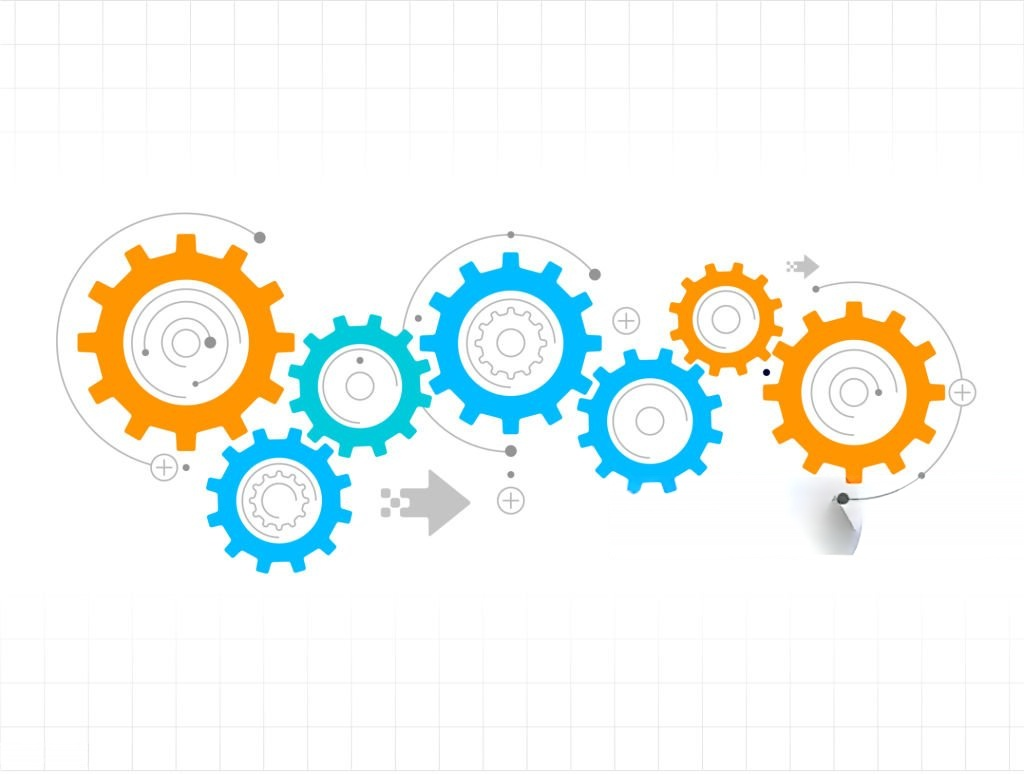
\includegraphics[width=0.85\textwidth]{images/architecture-diagrams/gear.jpeg}

    \floatcap{Modular Interlocking Logic Flow}{This diagram illustrates how the signal validator, rule engine, and DB layer interact during runtime.}
    
    \label{fig:micro-service-interaction}
\end{figure}


\section*{Signal Navigation Logic Flow}

The system determines signal state using the following flow:

\begin{enumerate}
  \item Validate current track and point statuses.
  \item Check dependent signals.
  \item Apply rule engine with selected control mode (AND/OR).
  \item Update signal aspect and record lock state.
\end{enumerate}

Additional flow diagrams or call graphs may be included.

\section*{Why This Architecture Outperforms Traditional Systems}

Our system:
\begin{itemize}
  \item Supports dynamic logic modes (AND/OR) for more flexibility.
  \item Separates validation and execution concerns (cleaner design).
  \item Introduces rule-based extensibility without modifying core logic.
\end{itemize}

Compared to traditional ladder-logic or static FSM designs, this approach offers better maintainability and modular expansion.


\end{appendices}

%% Bibliography:
\bibliographystyle{IEEEtran}
\bibliography{references}

\end{document}